
\title{ PyDash Architecture Document  \\ 
\includegraphics[width=2.50746in,height=2.26563in]{media/image24.jpg}}

\begin{longtable}[]{@{}ll@{}}
\toprule
\endhead
\begin{minipage}[t]{0.47\columnwidth}\raggedright
\textbf{PyDash 2018}

J. G. S. Overschie

T. W. E. Apol

A. Encinas-Rey Requena

K. Bolhuis

W. M. Wijnja

L. J. Doorenbos

J. Langhorst

A. Tilstra\strut
\end{minipage} & \begin{minipage}[t]{0.47\columnwidth}\raggedright
\textbf{Customers}

Patrick Vogel

Mircea Lungu

\textbf{TA}

Patrick Vogel\strut
\end{minipage}\tabularnewline
\bottomrule
\end{longtable}

\today

\pagebreak

\tableofcontents

\hypertarget{introduction}{%
\section{Introduction}\label{introduction}}

PyDash.io will be a platform for connecting existing Flask-monitoring
dashboards to and monitor those dashboards as well. This document will
describe the architecture and technologies used in the development of
the PyDash.io platform. It will also provide a short overview of the API
available.

There are several things this document focuses on, but they can be
categorized in a handful of segments. Each will deal with a part of the
design of PyDash.io. We will discuss the general architecture, tools
used, use-cases, back-end, front-end, our database and the API we built
for this piece of software.

\hypertarget{architectural-overview}{%
\section{Architectural Overview}\label{architectural-overview}}

The PyDash.IO application will be split into a couple of separate parts:

\begin{itemize}
\item
  \begin{quote}
  The Back-End part, which will be written using the Python programming
  language, and the Flask micro-web-framework.
  \end{quote}
\item
  \begin{quote}
  The Front-End part, which will be written as a Single-Page-Application
  using the React.JS interactive user interface framework.
  \end{quote}
\end{itemize}

These two parts will talk with each-other using a well-defined AJAX API
that will be outlined later in this document.

\hypertarget{use-cases}{%
\section{Use-Cases}\label{use-cases}}

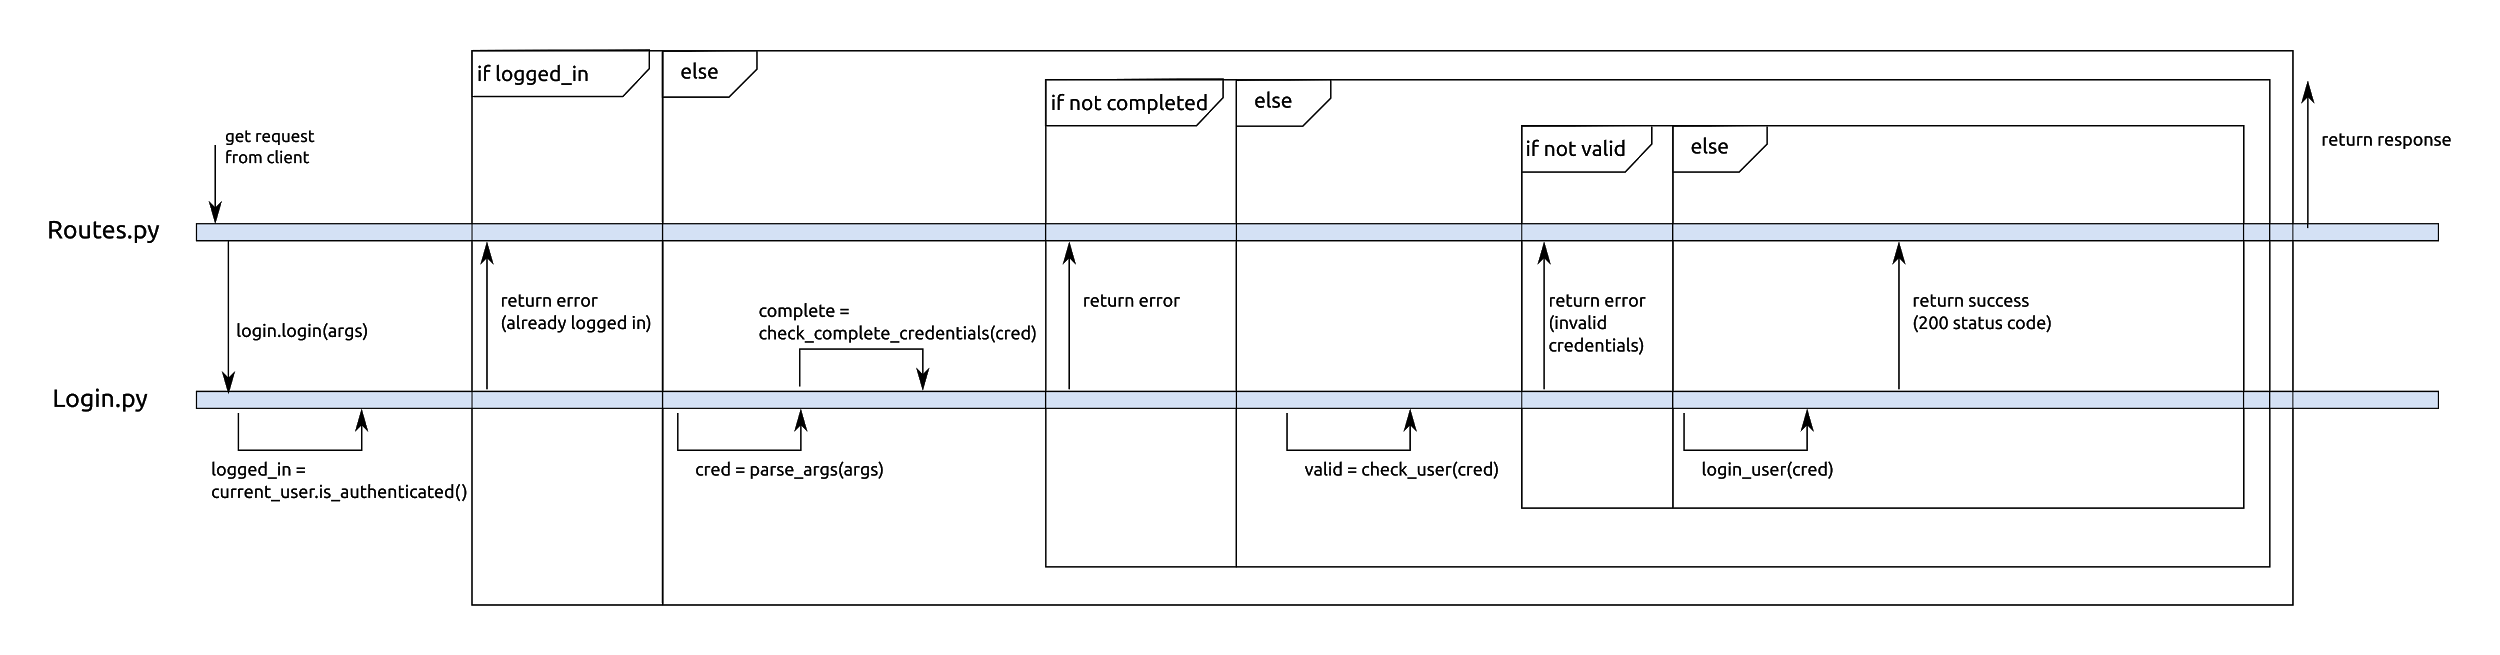
\includegraphics[width=\pagewidth]{media/image26.png}


\hypertarget{logging-in-to-pydash}{%
\subsection{Logging in to PyDash}\label{logging-in-to-pydash}}

If a user wants to use PyDash, he or she needs to be logged in to an
account. In order to log in the following steps have to be taken:

\textbf{Preconditions}

\begin{itemize}
\item
  \begin{quote}
  The account with which you want to log in exists in the database and
  you know the correct credentials for said account
  \end{quote}
\end{itemize}

\textbf{Postconditions}

\begin{itemize}
\item
  \begin{quote}
  The user is logged in to the correct account
  \end{quote}
\end{itemize}

\textbf{Main success scenario}

\begin{enumerate}
\def\labelenumi{\arabic{enumi}.}
\item
  \begin{quote}
  The user goes to the login page
  \end{quote}
\item
  \begin{quote}
  The user fills in the name and corresponding password
  \end{quote}
\item
  \begin{quote}
  The system successfully processes the request
  \end{quote}
\item
  \begin{quote}
  The user is redirected to his own dashboard overview page.
  \end{quote}
\end{enumerate}

\textbf{Alternative flow}

\begin{enumerate}
\def\labelenumi{\arabic{enumi}.}
\setcounter{enumi}{2}
\item
  \begin{quote}
  Incorrect credentials
  \end{quote}

  \begin{enumerate}
  \def\labelenumii{\alph{enumii}.}
  \item
    \begin{quote}
    The user is notified he entered the wrong credentials
    \end{quote}
  \item
    \begin{quote}
    Main success scenario continues at step 2.
    \end{quote}
  \end{enumerate}
\end{enumerate}

\hypertarget{registering-a-user}{%
\subsection{Registering a user}\label{registering-a-user}}

If a user wants to use PyDash, he or she needs an account. To create
such an account, a few steps have to be taken, which are described in
this use case.

\textbf{Preconditions}

\begin{itemize}
\item
  \begin{quote}
  None
  \end{quote}
\end{itemize}

\textbf{Postconditions}

\begin{itemize}
\item
  \begin{quote}
  The username-password combination is stored in the database
  \end{quote}
\item
  \begin{quote}
  An e-mail address is linked to the user
  \end{quote}
\end{itemize}

\textbf{Main success scenario}

\begin{enumerate}
\def\labelenumi{\arabic{enumi}.}
\item
  \begin{quote}
  The user requests to register an account
  \end{quote}
\item
  \begin{quote}
  The user fills in the necessary details (name, password, email)
  \end{quote}
\item
  \begin{quote}
  The system processes the request
  \end{quote}
\item
  \begin{quote}
  A verification email is sent to the newly registered user
  \end{quote}
\item
  \begin{quote}
  The user clicks the verification link in the email
  \end{quote}
\item
  \begin{quote}
  The user is notified of his successful account creation
  \end{quote}
\end{enumerate}

\textbf{Alternative flow}

\begin{enumerate}
\def\labelenumi{\arabic{enumi}.}
\setcounter{enumi}{1}
\item
  \begin{quote}
  Invalid combination, e.g. name is already taken.
  \end{quote}

  \begin{enumerate}
  \def\labelenumii{\alph{enumii}.}
  \item
    \begin{quote}
    The user is notified about what went wrong
    \end{quote}
  \item
    \begin{quote}
    Main success scenario continues at step 2.
    \end{quote}
  \end{enumerate}
\end{enumerate}

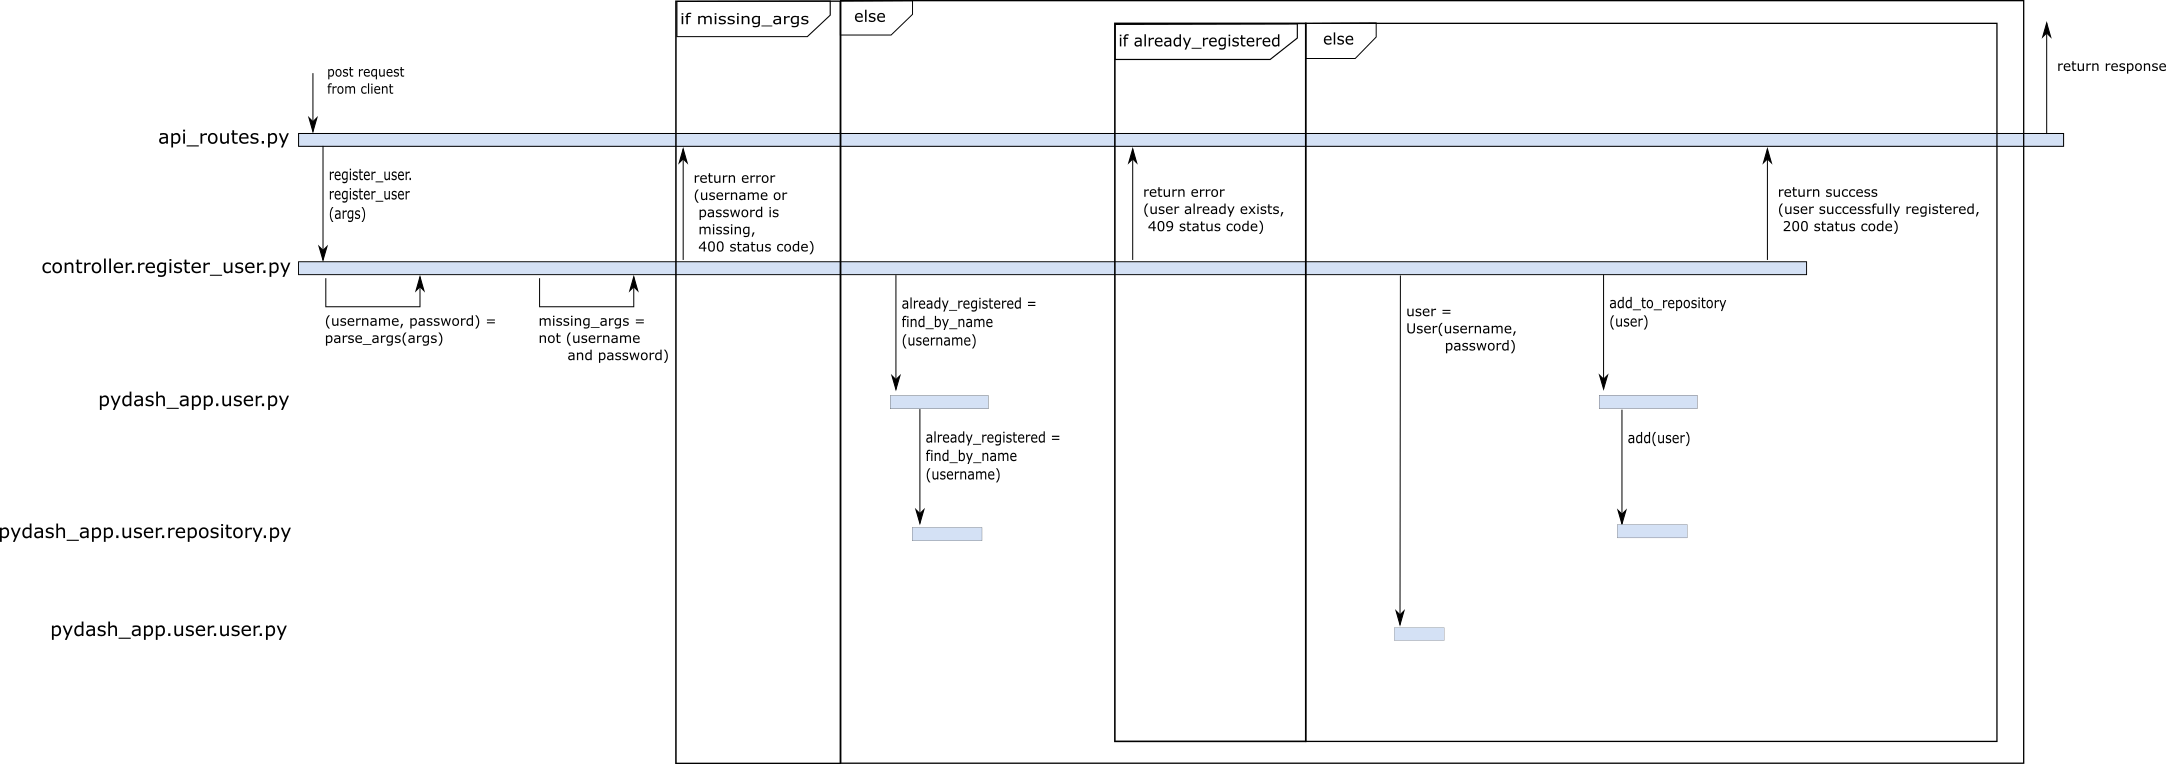
\includegraphics[width=\pagewidth]{media/image21.png}

\hypertarget{viewing-the-data-of-a-certain-dashboard}{%
\subsection{Viewing the data of a certain
dashboard}\label{viewing-the-data-of-a-certain-dashboard}}

This use case describes the process of a user wanting to view the flask
monitoring dashboard data of a certain site.

\textbf{Preconditions}

\begin{itemize}
\item
  \begin{quote}
  The user is logged in
  \end{quote}
\item
  \begin{quote}
  The dashboard of which the data will be viewed is linked to the user
  \end{quote}
\end{itemize}

\textbf{Postconditions}

\begin{itemize}
\item
  \begin{quote}
  The correct data of the correct dashboard is presented to the user in
  a readable fashion
  \end{quote}
\end{itemize}

\textbf{Main success scenario}

\begin{enumerate}
\def\labelenumi{\arabic{enumi}.}
\item
  \begin{quote}
  The user selects the dashboard for which he wants to see the data
  \end{quote}
\item
  \begin{quote}
  Optionally the user filters out the endpoints he is not interested in
  \end{quote}
\item
  \begin{quote}
  The system retrieves the correct dashboard and displays the data
  \end{quote}
\end{enumerate}

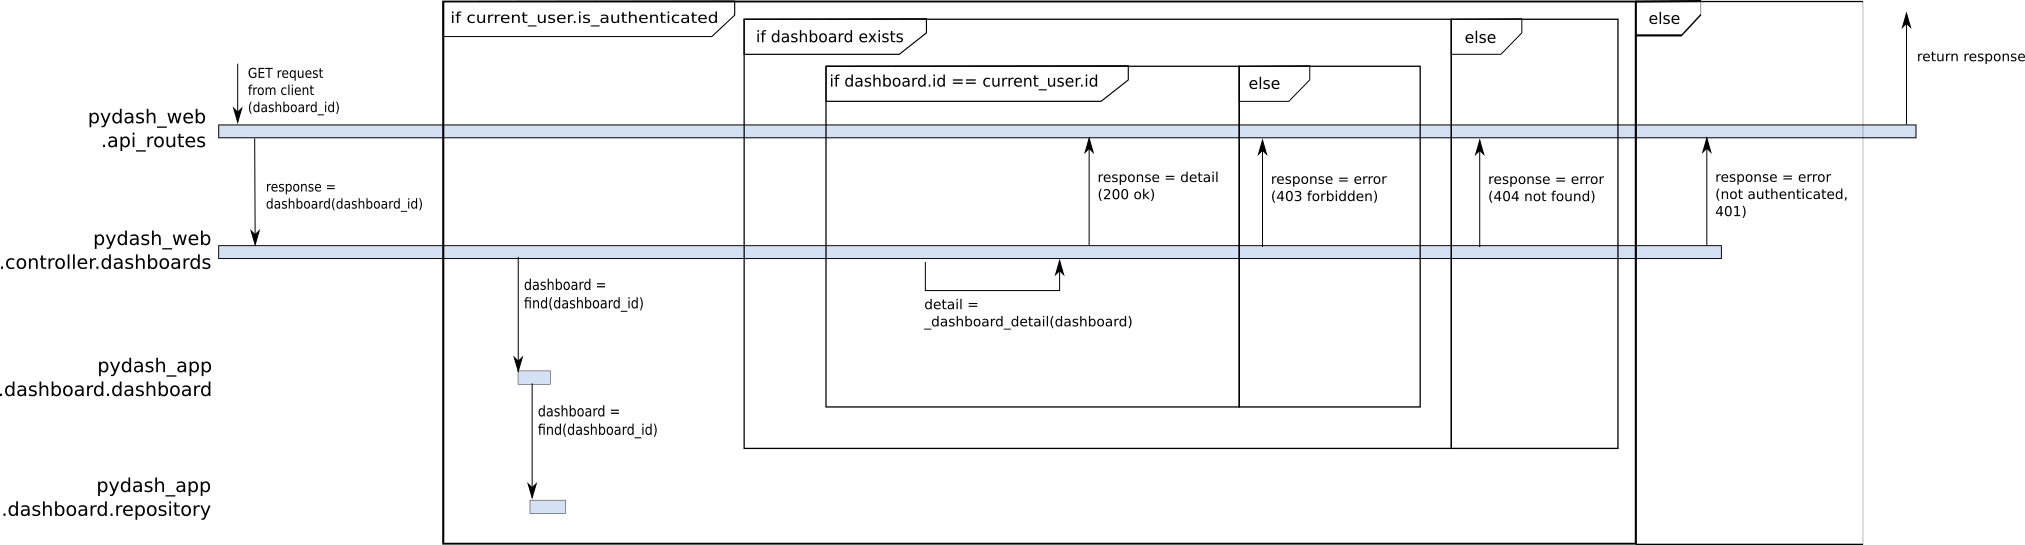
\includegraphics[width=\pagewidth]{media/image30.png}

\hypertarget{registering-a-dashboard}{%
\subsection{Registering a dashboard}\label{registering-a-dashboard}}

PyDash gathers data of multiple flask monitoring dashboards, but to do
so they first have to be added by the user to his meta dashboard. This
use case describes this process of adding a new dashboard to your
overview.

\textbf{Preconditions}

\begin{itemize}
\item
  \begin{quote}
  The user is logged in
  \end{quote}
\item
  \begin{quote}
  The user is in possession of the secret token associated with that
  dashboard
  \end{quote}
\end{itemize}

\textbf{Postconditions}

\begin{itemize}
\item
  \begin{quote}
  The corresponding dashboard is added to the user's overview
  \end{quote}
\end{itemize}

\textbf{Main success scenario}

\begin{enumerate}
\def\labelenumi{\arabic{enumi}.}
\item
  \begin{quote}
  The user clicks the plus sign, the button for registering a new
  dashboard
  \end{quote}
\item
  \begin{quote}
  The user fills in the url, the name he wants and the secret token
  associated with that dashboard
  \end{quote}
\item
  \begin{quote}
  The system checks if the token and url combination is correct
  \end{quote}
\item
  \begin{quote}
  The new dashboard is added to the overview page
  \end{quote}
\end{enumerate}

\textbf{Alternative flow}

\begin{enumerate}
\def\labelenumi{\arabic{enumi}.}
\setcounter{enumi}{2}
\item
  \begin{quote}
  The token/url combination is incorrect
  \end{quote}

  \begin{enumerate}
  \def\labelenumii{\alph{enumii}.}
  \item
    \begin{quote}
    The user is notified that the given combination is wrong
    \end{quote}
  \item
    \begin{quote}
    Main success scenario continues at step 2.
    \end{quote}
  \end{enumerate}
\end{enumerate}

\hypertarget{back-end-design}{%
\section{Back-end Design}\label{back-end-design}}

The Back-End part of the application is written in Python using the
Flask micro-web-framework. The reason to use Flask here is to be able to
use the \emph{flask-monitoring-dashboard}, a Python library whose
functionality PyDash.IO builds on top of, to be used for the
\emph{PyDash.IO} web-application itself as well.

The Back-End is split up using the well-known
\emph{Model-View-Controller} architecture pattern.

The \emph{Model} contains all the actual application logic. Its
implementation can be found in the \emph{pydash\_app} folder. The
web-application is only a consumer of this package.

The \emph{Controller} contains the dispatching logic to know how to
respond to the different endpoints a visitor might request. The actual
route-dispatching happens in \emph{pydash\_web/api\_routes.py} , with
the handling of each of the different routes being handled by its own
dedicated module in the \emph{pydash\_web/controller/} folder.

The \emph{View} part of the application currently consists of the
\emph{api\_routes.py} file. This file serves as an interface between the
front-end and back-end, thus being the view of the back-end with regards
to the outside world.

\hypertarget{domain-driven-design}{%
\subsection{Domain Driven Design}\label{domain-driven-design}}

Inside the application logic (\emph{pydash\_app}), we use a simple
variant of Domain Driven Design to split up our model's functionality in
their respective concerns. For each data structure or
finite-state-machine of interest, we create three parts:

\begin{enumerate}
\def\labelenumi{\arabic{enumi}.}
\item
  \begin{quote}
  A module of the entity name that contains the publicly available
  functions to interact with these entities.
  \end{quote}
\item
  \begin{quote}
  A \emph{Repository} module that knows how entities of this type are
  persisted: It exposes functionality to find certain entities of this
  type in the persistence layer, create new ones, update existing ones
  and possibly delete them. Only the actions that are actually relevant
  to the specific entities are modeled. The Repository is the only part
  that actually talks with the underlying persistence layer, and as such
  it can be considered an Adapter.
  \end{quote}
\item
  \begin{quote}
  An \emph{Entity} class which is a plain Python class with the
  properties of interest and the methods that make sense to prove and
  possibly manipulate this kind of entity.
  \end{quote}
\end{enumerate}

Important to note is thus:

The Entity never knows how it itself is persisted,

The Repository does not care about the internals of the Entity's logic.

Because of this, both are easy to change without needing to touch the
other.

\hypertarget{database-design}{%
\subsection{Database Design}\label{database-design}}

We have decided on using the ZODB object-database as it provides a clear
relationship between objects and elements in the database. ZODB in
essence uses a large tree-like structure to store Python objects. Each
class has its own branch which is a set of objects of that class. Each
of these branches is called a repository.

To connect to ZODB we use ZEO. This is a tool that allows the database
to be ran in a separate process to not poorly influence the performance
of the web-app.

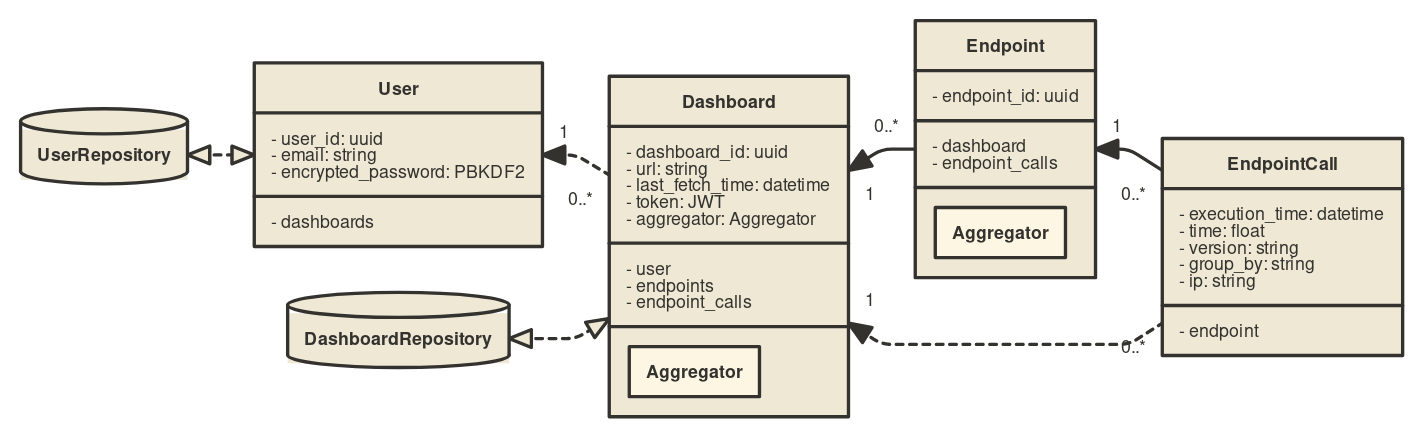
\includegraphics[width=\pagewidth]{media/image31.png}

\hypertarget{section-6}{%
\section{\texorpdfstring{\\
}{ }}\label{section-6}}

\hypertarget{front-end-design}{%
\section{Front-end Design}\label{front-end-design}}

For the front-end part of the application, we will be creating a
one-page application using the React.js framework, requesting all
necessary information from the back-end using AJAX (Asynchonous
Javascript and XML) calls.

For the User interface, we will be using the Material-UI framework, with
the pages looking like this:

For the time being, there will be a few different pages:

\begin{itemize}
\item
  \begin{quote}
  The landing page/login page: When the users enter the website, this
  will be the first page they see. They will be able to login to an
  existing account.
  \end{quote}
\end{itemize}

\emph{The login page will look approximately like this.}

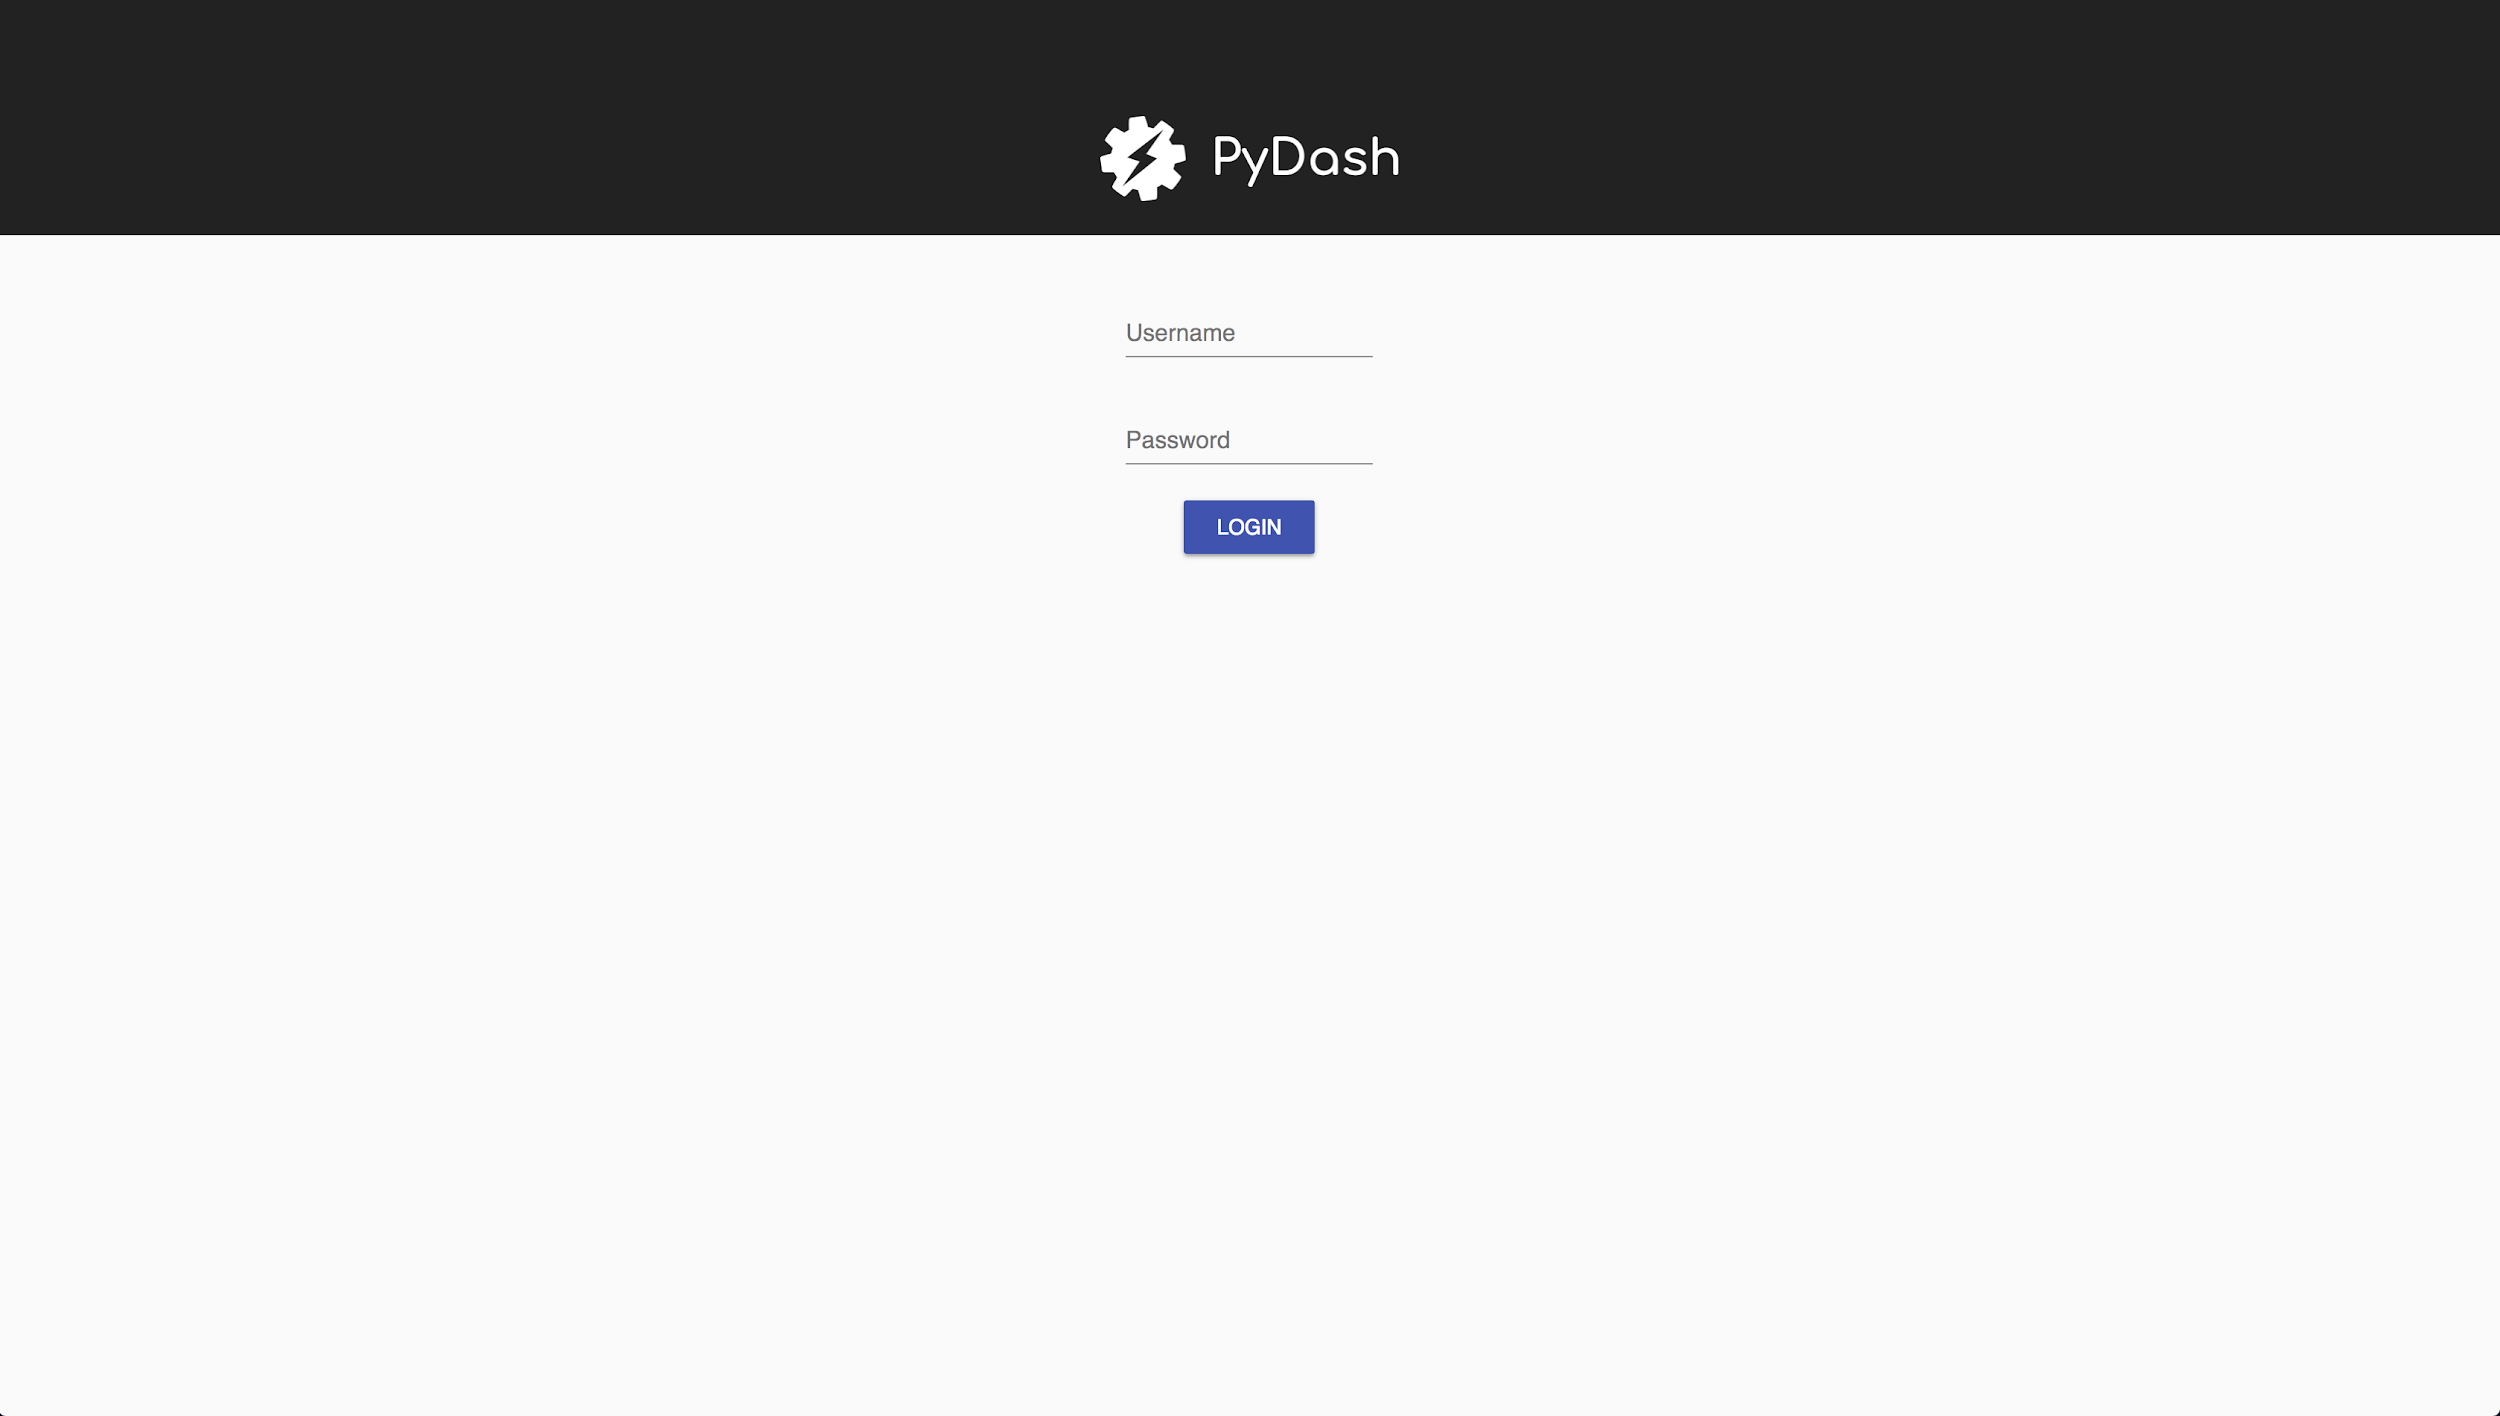
\includegraphics[width=\pagewidth]{media/image28.png}

\begin{itemize}
\item
  \begin{quote}
  The overview page: Here the users will be able to see an overview of
  all dashboards they are monitoring.
  \end{quote}
\end{itemize}

\emph{The overview page will look approximately like
this.}

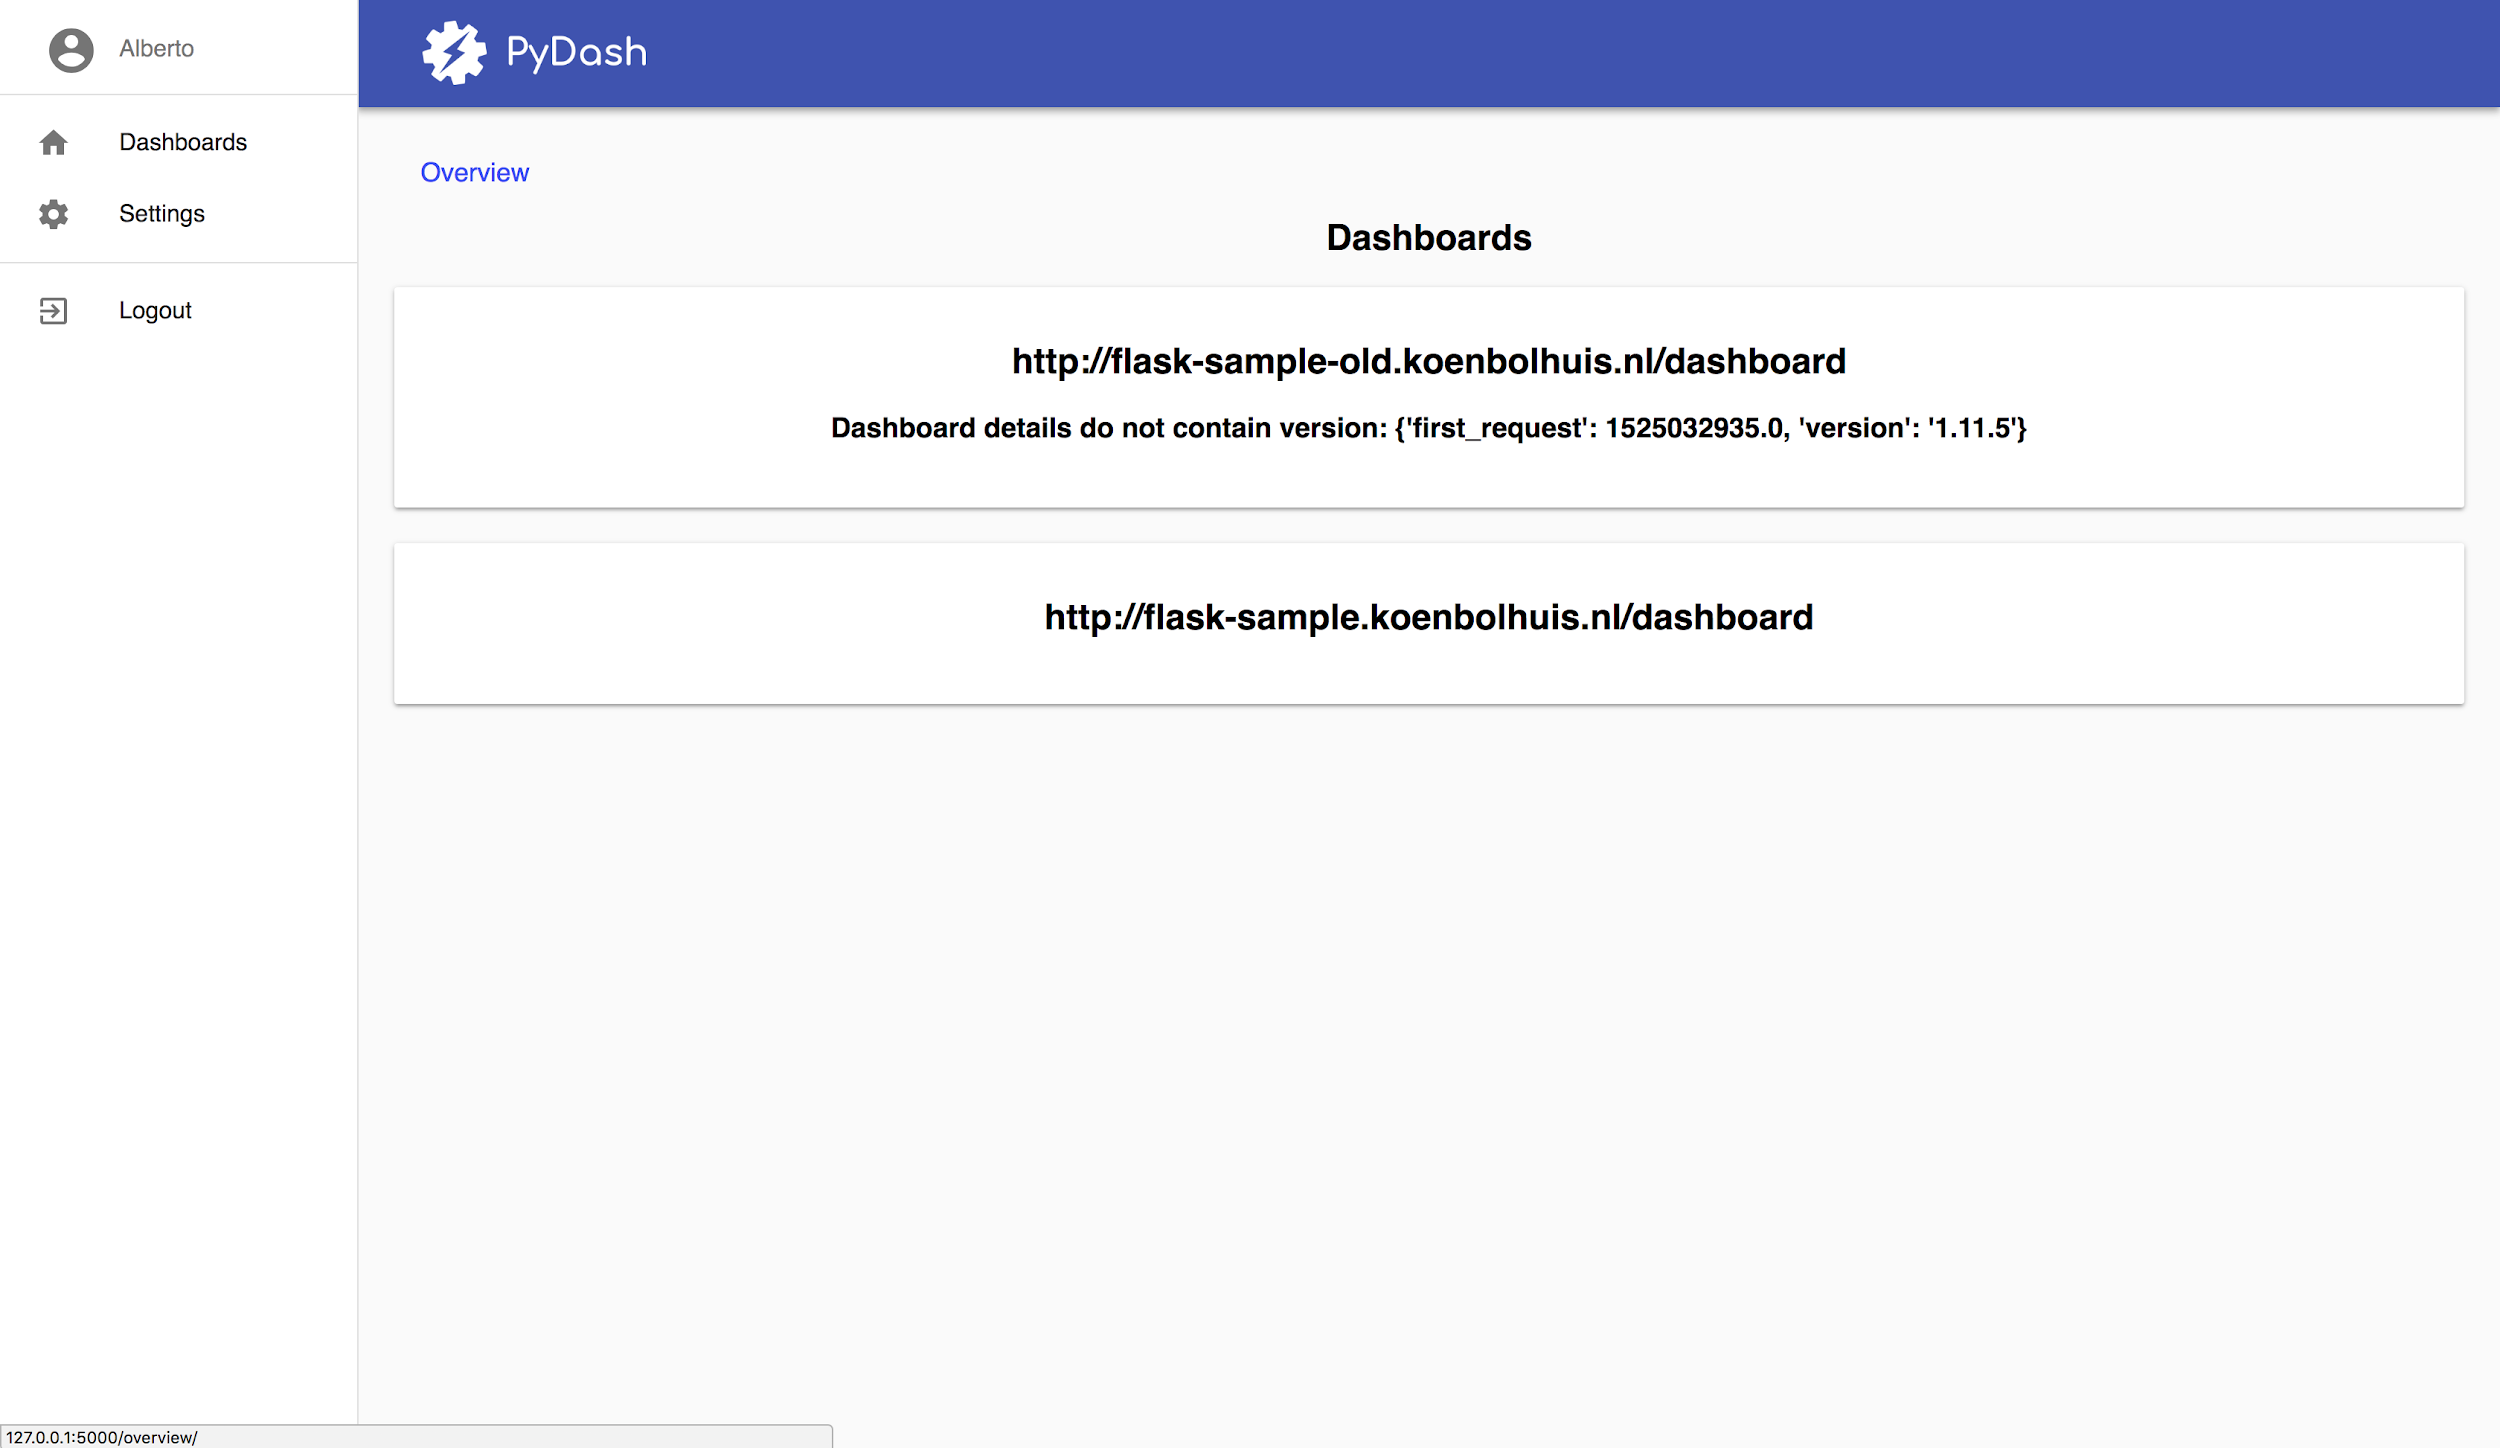
\includegraphics[width=\pagewidth]{media/image33.png}

\begin{itemize}
\item
  \begin{quote}
  The dashboard page (Here the users will be able to see all
  information coming in from the specified dashboard.
  \end{quote}
\end{itemize}

\emph{The dashboard page will look approximately like
this.}

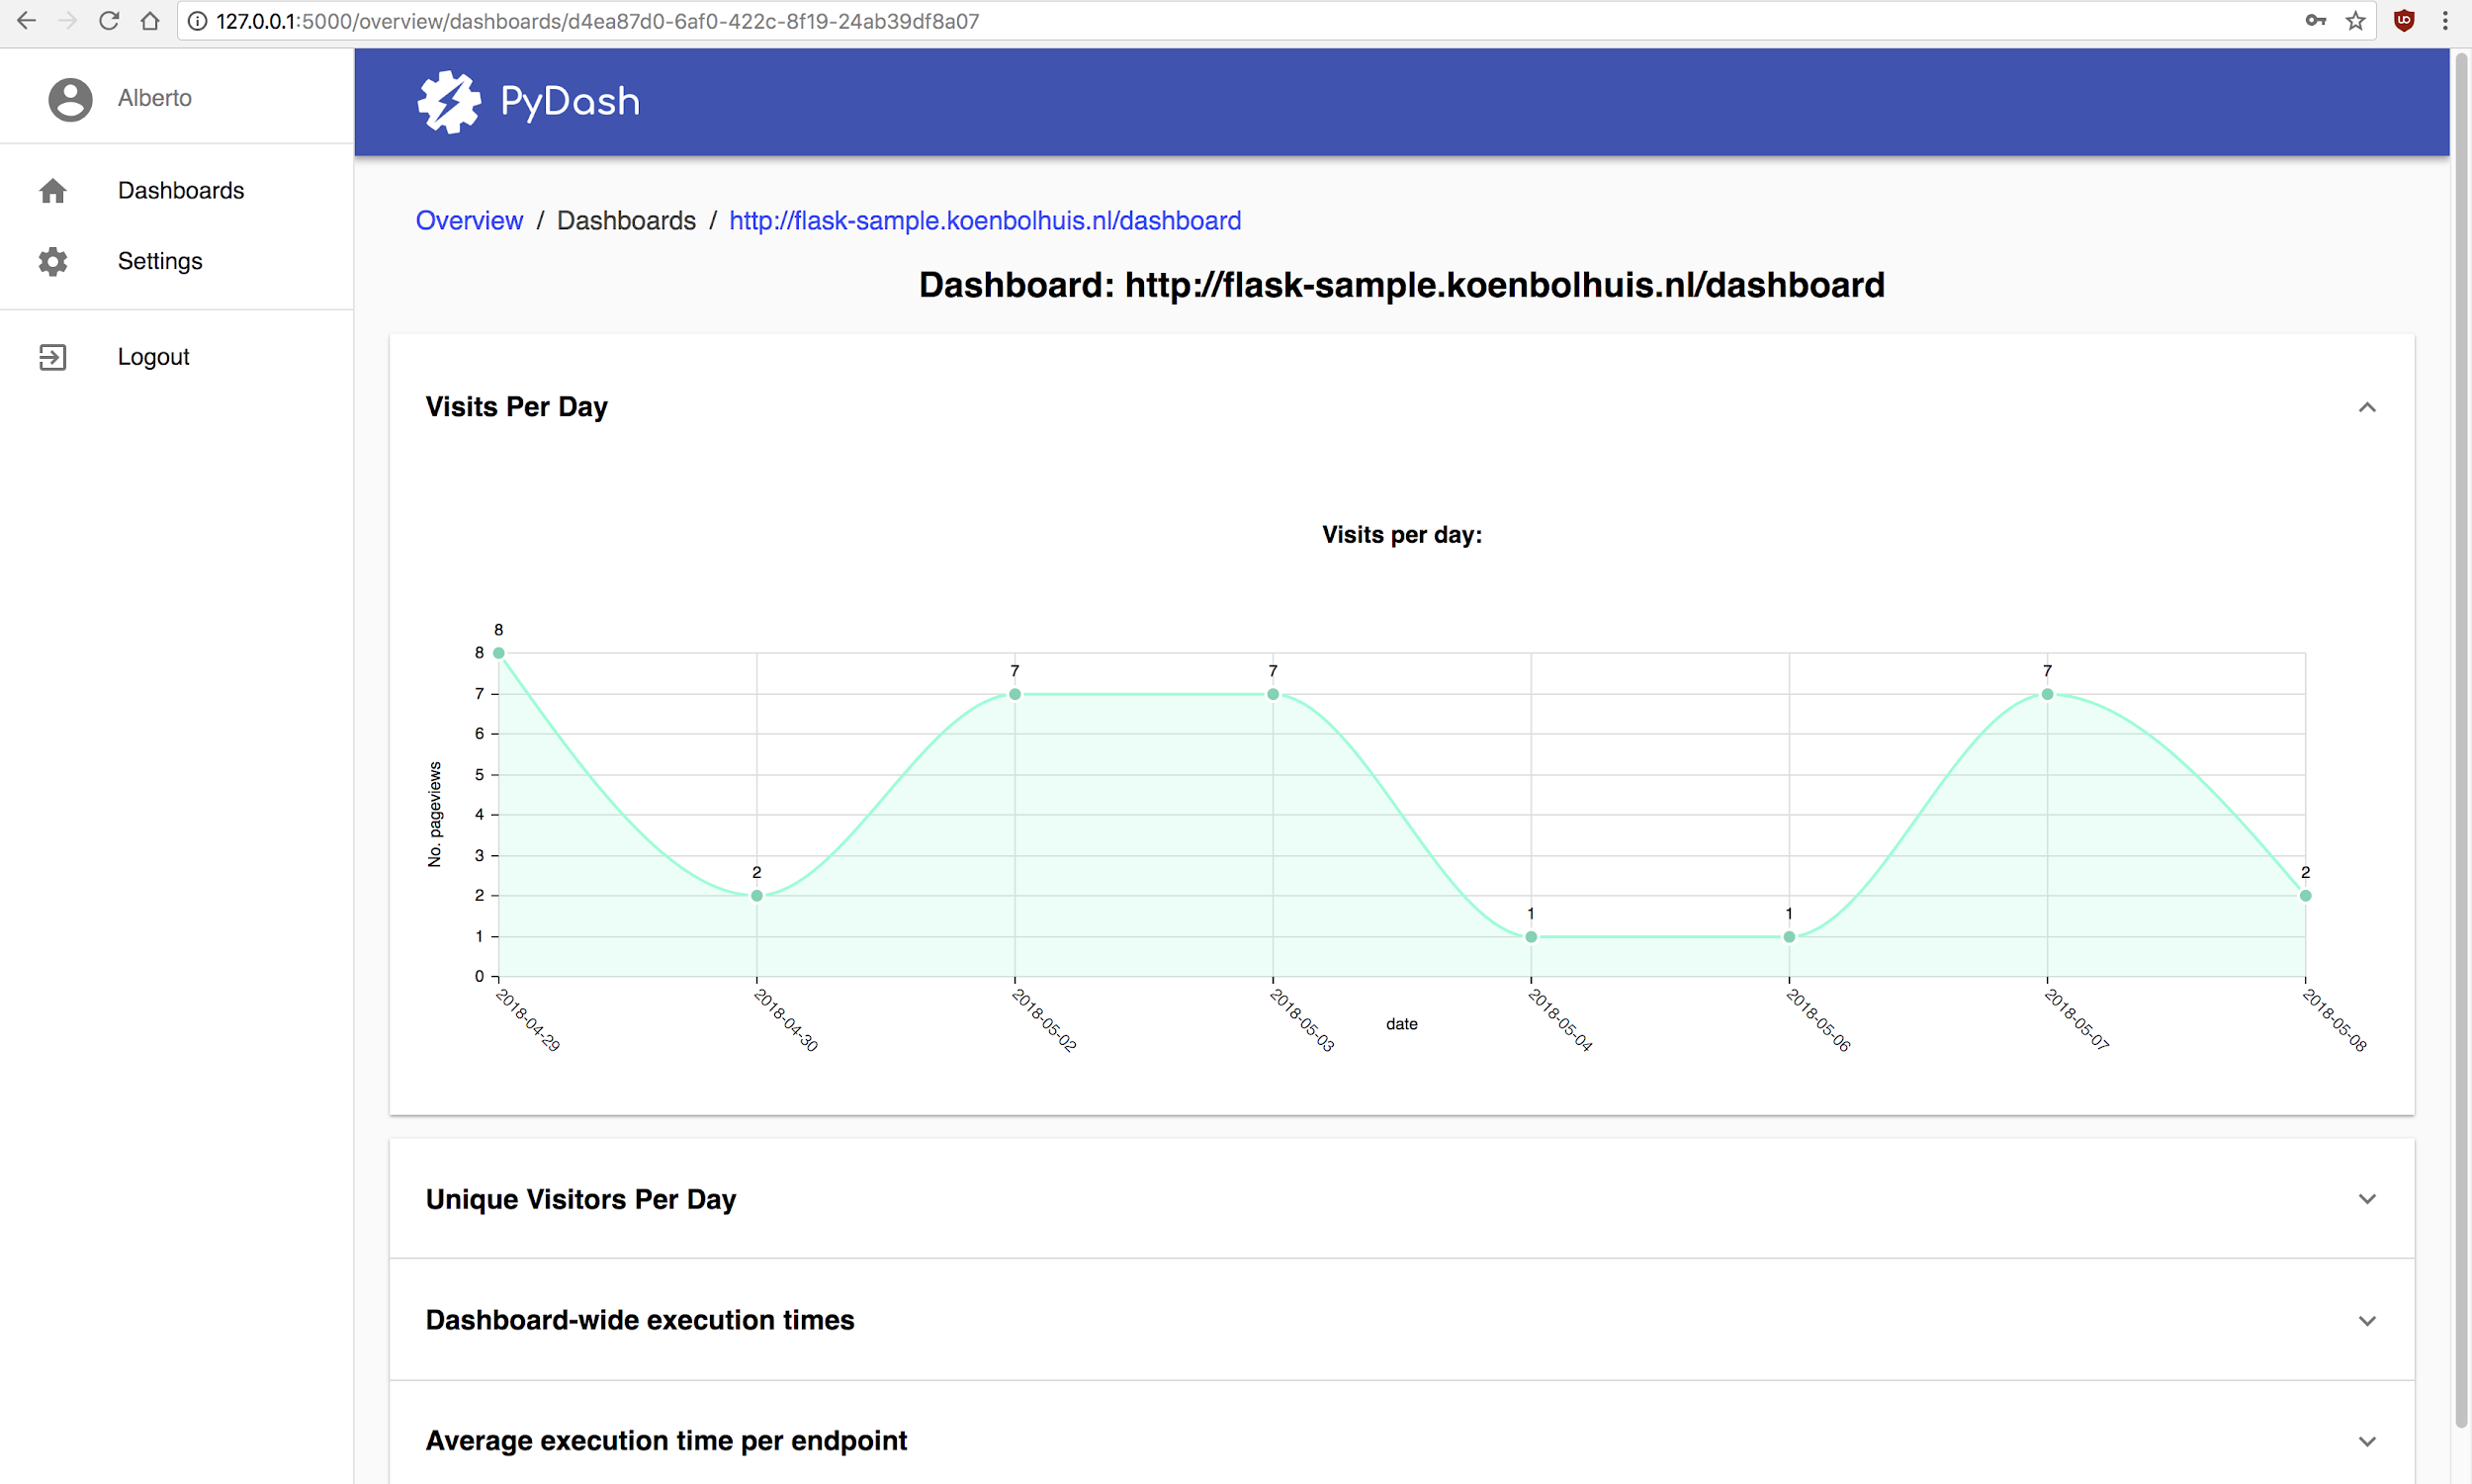
\includegraphics[width=\pagewidth]{media/image27.png}

\begin{itemize}
\item
  \begin{quote}
  The register page: Here the users will be able to create a new account
  \end{quote}
\end{itemize}

\emph{The registration page will look approximately like
this.}

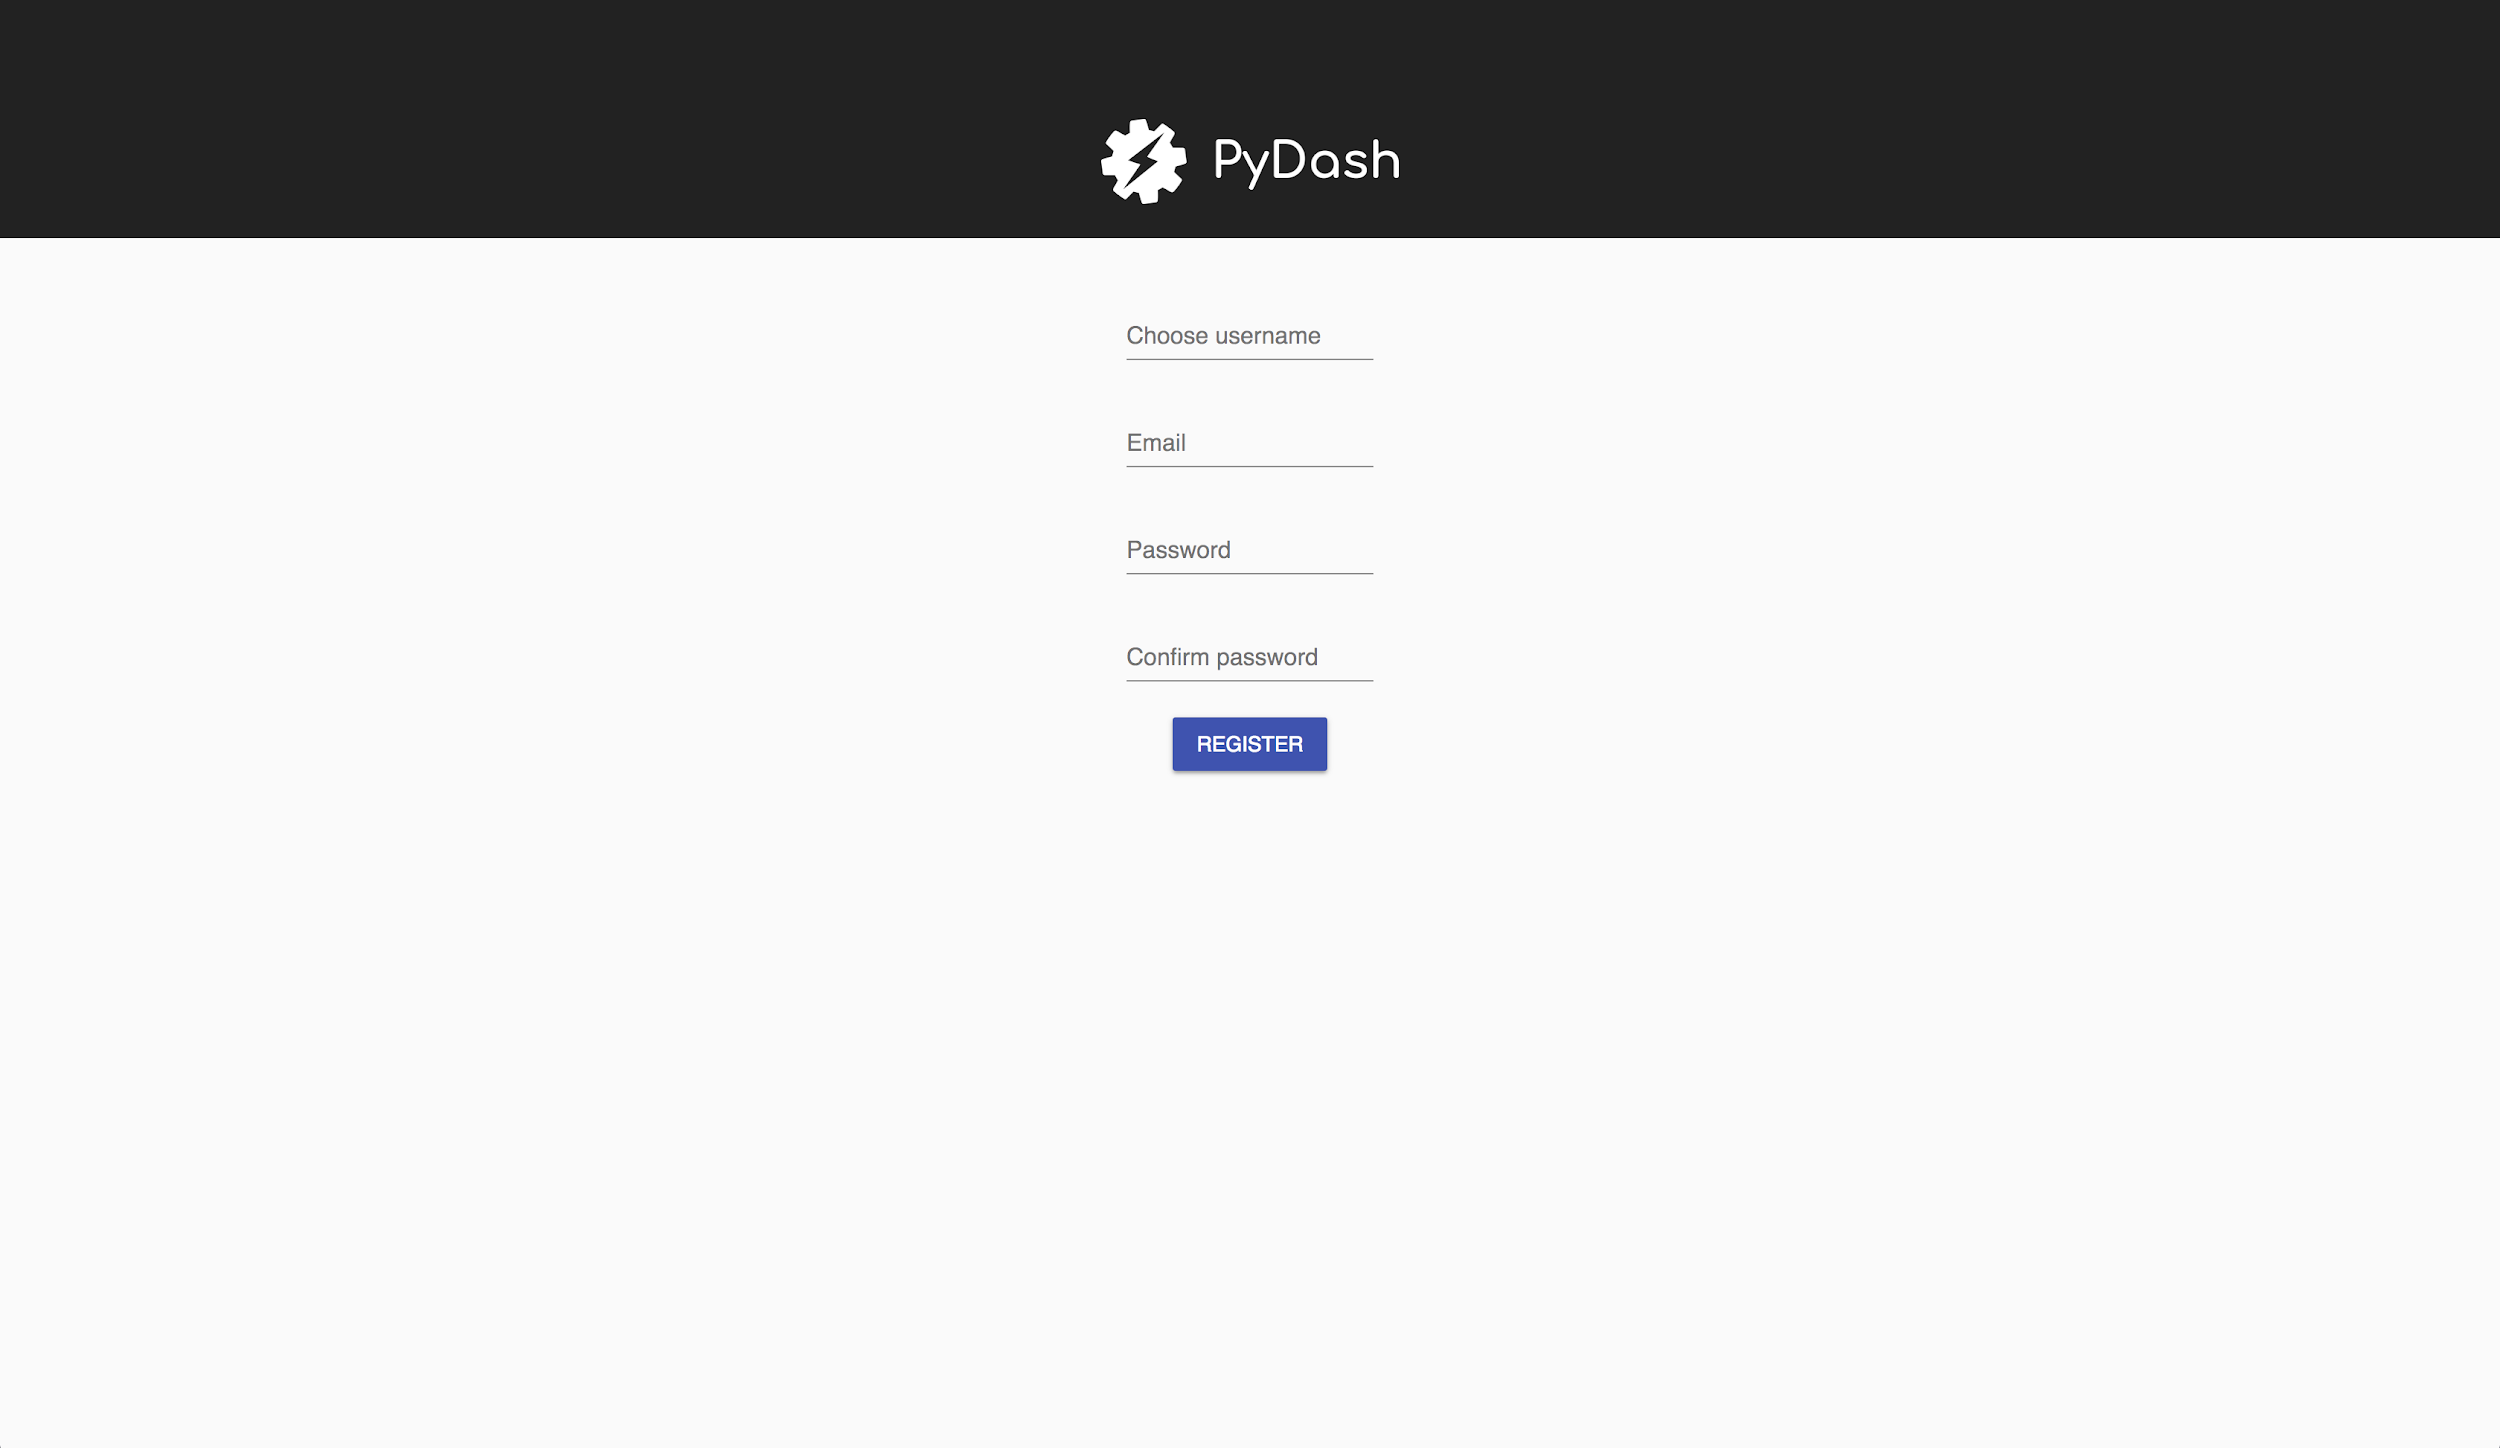
\includegraphics[width=\pagewidth]{media/image40.png}

\begin{itemize}
\item
  \begin{quote}
  Add dashboard: Here the users will be able to create a new dashboard
  by pressing a button located on the top right corner which opens a
  form to create the dashboard.
  \end{quote}
\end{itemize}

\emph{The add dashboard page will look approximately like this.}

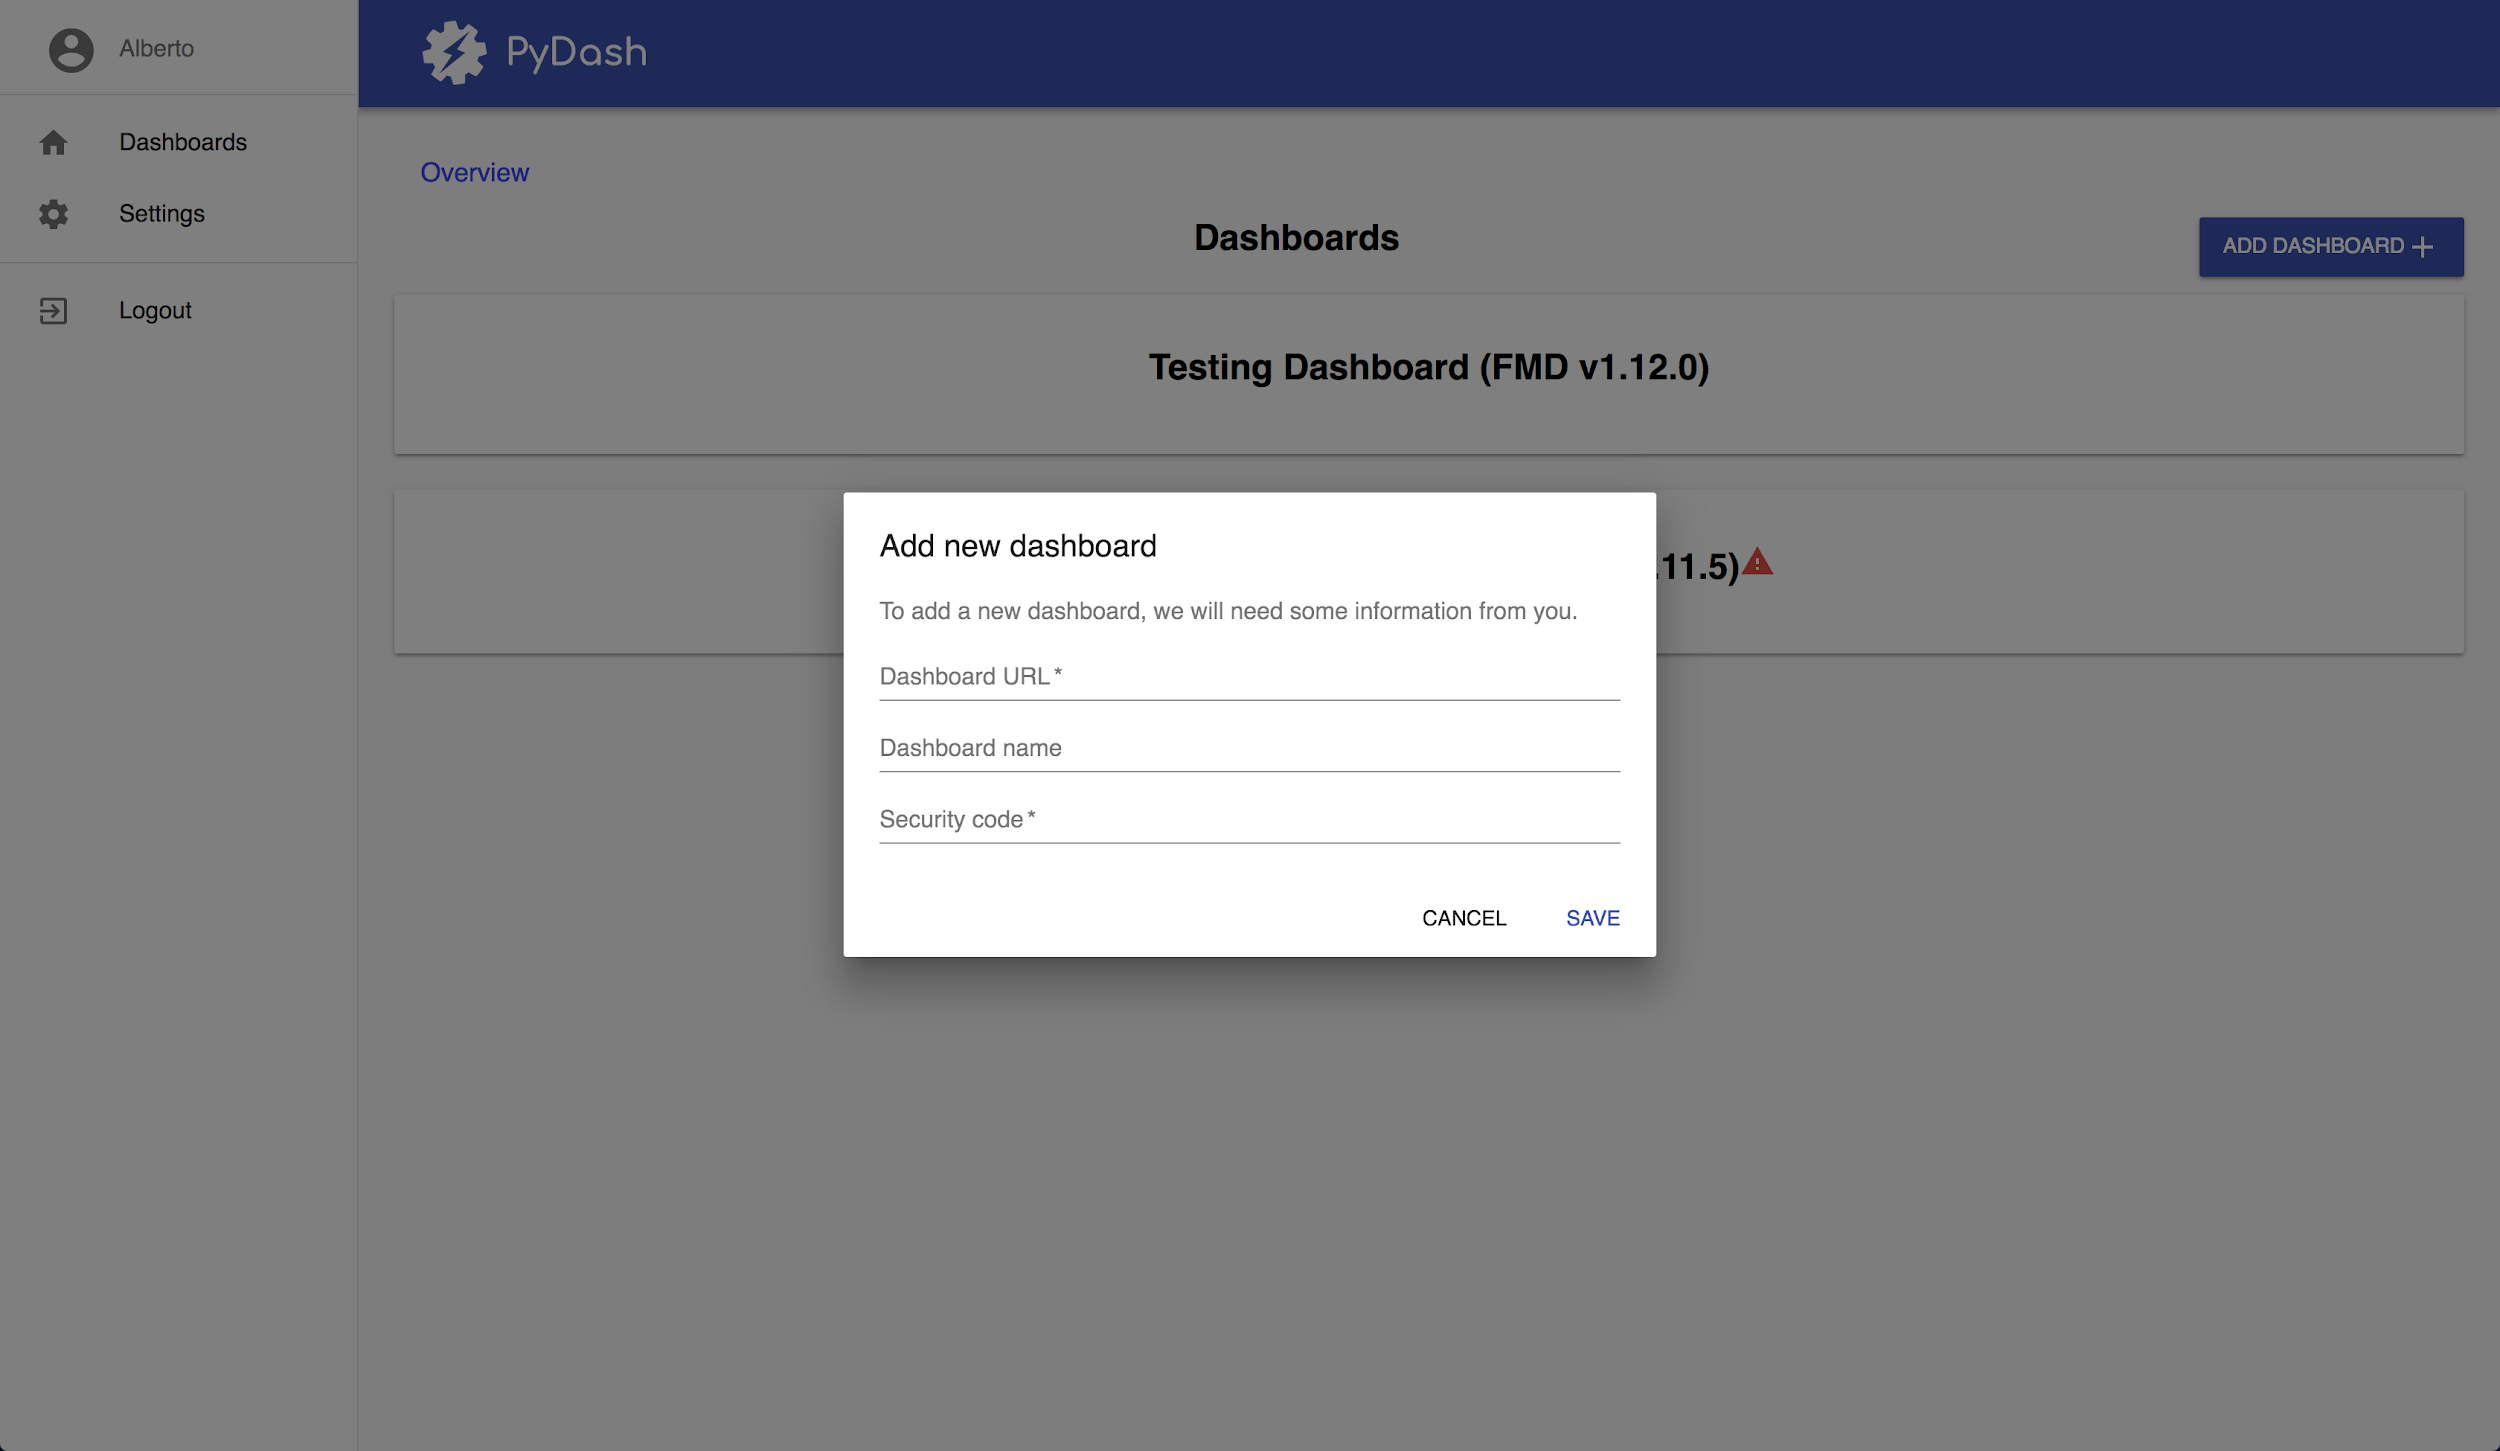
\includegraphics[width=\pagewidth]{media/image25.png}

\begin{itemize}
\item
  \begin{quote}
  The settings page: Here the users will be able to edit or erase their
  accounts by changing their username, password or email inside a dialog
  form. As well as that the user will be allowed to turn of the sounds.
  It consists on expandable panels.
  \end{quote}
\end{itemize}

\emph{The settings page will look approximately like this.}


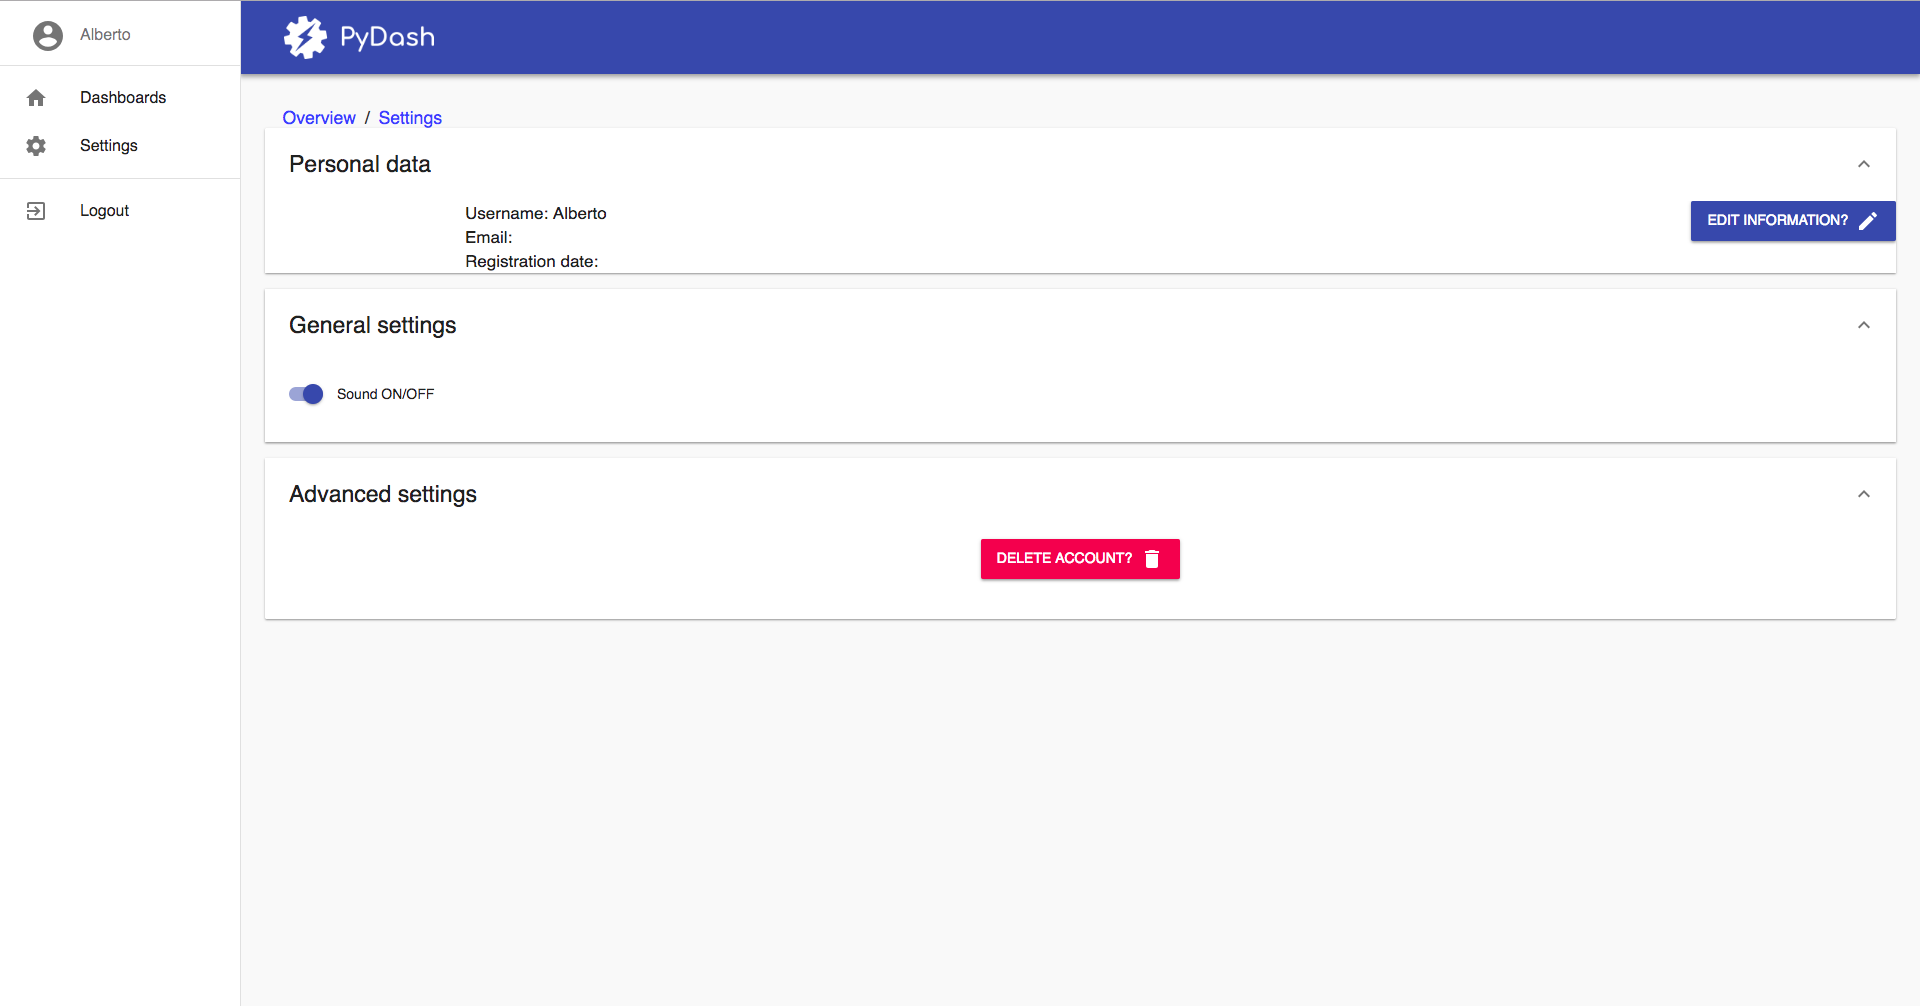
\includegraphics[width=\pagewidth]{media/image38.png}


\hypertarget{back-end-technology-stack}{%
\subsection{Back-End Technology Stack}\label{back-end-technology-stack}}

In the Back-End of the Pydash.IO application, we have attempted to keep
the number of moving parts as small as possible, because adding more
things makes it increasingly difficult to set up the codebase on a new
server and to maintain it all because of the mental overhead to
understand a large group of tools at the same time.

This is the main reason we decided \emph{not} to use an SQL database,
but instead a Python Object Database, which allows us to just work
directly with Python objects. It is also the reason we do not use the
common library Celery for background-task-management (which requires an
externally-running in-memory database like Redis) but instead created
our own simple task scheduler that directly works inside Python 3.

\begin{itemize}
\item
  \begin{quote}
  \textbf{Python 3:} The Programming Language which everything is built
  in. Python is an object-oriented programming language (with influences
  from functional programming) that has a large ecosystem of people
  providing free and open-source libraries to help with all kinds of
  tasks.
  \end{quote}
\item
  \begin{quote}
  \textbf{Flask:} The 'micro' web-framework built on top of Python,
  which makes it very clear to the developer what is going on (rather
  than doing all kinds of magic behind the scenes).
  \end{quote}
\item
  \begin{quote}
  \textbf{PyJWT} is used to work with JSON-WEB-Tokens which
  encrypt/decrypt the communication between the remote
  flask-monitoring-dashboards over a potentially unsafe (i.e.
  \emph{http}) connection.
  \end{quote}
\item
  \begin{quote}
  \textbf{Zope Object Database} (exposed using ZEO): The database-layer
  we use to persist Python-objects in. We have created a custom
  indexable dictionary-like structure that allows us to easily search
  for certain objects on top of this (This has been split off in the
  Python package \textbf{multi-indexed-collection}). Using an Object
  Database means that we do not require to think about the peculiarities
  of an object-relational-mapping tool.
  \end{quote}
\item
  \begin{quote}
  \textbf{Custom Periodic Task scheduler:} A custom piece of code that
  schedules tasks using a pool of Subprocesses. This means that
  background- and periodic tasks will always run quickly without
  impacting the people that perform a request to the Flask application.
  The actual task scheduler is built in such a way that only the minimum
  of work is done to check what tasks should be run shortly.
  (internally, an indexable priority queue is used for this).
  \end{quote}
\end{itemize}

\hypertarget{front-end-technology-stack}{%
\subsection{Front-End Technology
stack}\label{front-end-technology-stack}}

We use a lot of different technologies in the Front-End. Mainly, we
follow some of the conventions used in the React build tool
\href{https://github.com/facebook/create-react-app/}{{create-react-app}}.
Technologies we use include:

\begin{longtable}[]{@{}ll@{}}
\toprule
\begin{minipage}[b]{0.47\columnwidth}\raggedright

\includegraphics[width=0.77633in,height=0.77633in]{media/image22.png}

webpack\strut
\end{minipage} & \begin{minipage}[b]{0.47\columnwidth}\raggedright
Webpack gives us a nice way to pack up our application for production
usage. It takes all your javascript modules, and recursively iterates
through its dependencies, which enables us to exactly only include the
modules that we actually use. This makes for no redundant code, and a
nice packaged up single file with your application. It does the same for
you with CSS. It also compresses images, along with some other nice
stuff.

* Module-bundling

* Asset compression

* Code minification\strut
\end{minipage}\tabularnewline
\midrule
\endhead
\begin{minipage}[t]{0.47\columnwidth}\raggedright

\includegraphics[width=0.77633in,height=0.77633in]{media/image39.png}

LiveReload\strut
\end{minipage} & \begin{minipage}[t]{0.47\columnwidth}\raggedright
LiveReload enables us to have a fast development cycle by automatically
reloading the browser page upon saving a file from the project. This is
done by efficiently monitoring the project filesystem folder.

* Fast development

cycle\strut
\end{minipage}\tabularnewline
\begin{minipage}[t]{0.47\columnwidth}\raggedright

\includegraphics[width=0.74114in,height=0.74114in]{media/image32.png}

ESLint\strut
\end{minipage} & \begin{minipage}[t]{0.47\columnwidth}\raggedright
ESLint scans our javascript for common flaws and warns you about them
right in your text editor. Common flaws include warning about unused
variables, unreachable code, messy assignments or weird constructs. It
improves your code quality greatly overall. Aside from warnings in your
editor it also warns you on the command line in the build process.

* Find errors

early\strut
\end{minipage}\tabularnewline
\begin{minipage}[t]{0.47\columnwidth}\raggedright

\includegraphics[width=0.66371in,height=0.66371in]{media/image34.png}

JSX\strut
\end{minipage} & \begin{minipage}[t]{0.47\columnwidth}\raggedright
JSX is a widely used precompiled dialect of Javascript in React.js. It
allows mixed usage of HTML and JS in one file without too much syntactic
overhead.

* Write HTML

in JS

* Cleaner code\strut
\end{minipage}\tabularnewline
\begin{minipage}[t]{0.47\columnwidth}\raggedright

\includegraphics[width=1.36082in,height=0.61811in]{media/image36.png}

babel\strut
\end{minipage} & \begin{minipage}[t]{0.47\columnwidth}\raggedright
Babel allows us to write next-generation JavaScript! Nowadays most JS
developers write JS using the ES6 (and higher) standards. Babel allows
compiling this modern JS syntax to browser-compatible JavaScript.

* Modern JS\strut
\end{minipage}\tabularnewline
\begin{minipage}[t]{0.47\columnwidth}\raggedright

\includegraphics[width=0.77633in,height=0.77633in]{media/image37.png}

Service Worker\strut
\end{minipage} & \begin{minipage}[t]{0.47\columnwidth}\raggedright
Create-react-app automatically hooks up a service-worker for you, which
allows offline-usage and asset caching for your app.

* Cache

assets\strut
\end{minipage}\tabularnewline
\begin{minipage}[t]{0.47\columnwidth}\raggedright

\includegraphics[width=0.34896in,height=0.34896in]{media/image23.png}

github.com/axios\strut
\end{minipage} & \begin{minipage}[t]{0.47\columnwidth}\raggedright
Axios is the AJAX library we use to make HTTP calls in React. For every
piece of retrieved JSON data, we send an AJAX request to our backend
using Axios.\strut
\end{minipage}\tabularnewline
\begin{minipage}[t]{0.47\columnwidth}\raggedright

\includegraphics[width=1.44761in,height=1.17188in]{media/image29.png}

Material-UI\strut
\end{minipage} & \begin{minipage}[t]{0.47\columnwidth}\raggedright
Material-ui is the interface library we use. It is based upon the
Material Design principles from Google, and has bindings for React.js.
Bindings allow you to easily observe and bind Javascript variables to
text in the view.

* No need to create UI components ourselves.\strut
\end{minipage}\tabularnewline
\begin{minipage}[t]{0.47\columnwidth}\raggedright

\includegraphics[width=2.08854in,height=0.65523in]{media/image35.png}

NIVO\strut
\end{minipage} & \begin{minipage}[t]{0.47\columnwidth}\raggedright
We use NIVO for displaying graphs in our statistics page. NIVO has an
elaborate library of default graphs you can use. Customization is easy
to do if wanted, NIVO's defaults are really good as well, though.\strut
\end{minipage}\tabularnewline
\bottomrule
\end{longtable}

\hypertarget{section-18}{%
\section{\texorpdfstring{\\
}{ }}\label{section-18}}

\hypertarget{api-specification}{%
\section{API Specification}\label{api-specification}}

\emph{an * (asterisk) indicates that a certain parameter is mandatory.}

\hypertarget{user}{%
\subsection{User}\label{user}}

\hypertarget{apilogin}{%
\subsubsection{/api/login}\label{apilogin}}

Logs a user into the system.

\begin{itemize}
\item
  \begin{quote}
  *name (string) - Name of the user to be logged in.
  \end{quote}
\item
  \begin{quote}
  *password (string) - Password for login in clear text.
  \end{quote}
\end{itemize}

Responses:

\begin{itemize}
\item
  \begin{quote}
  200 - User was logged in correctly.
  \end{quote}
\item
  \begin{quote}
  400 - Missing username or password.
  \end{quote}
\item
  \begin{quote}
  401 - Invalid username/password supplied.
  \end{quote}
\end{itemize}

\hypertarget{apilogout}{%
\subsubsection{/api/logout}\label{apilogout}}

Logs the current user out.

\emph{No parameters required}

Responses:

\begin{itemize}
\item
  \begin{quote}
  200 - Successful operation.
  \end{quote}
\item
  \begin{quote}
  401 - Returned if user was not logged in.
  \end{quote}
\end{itemize}

\hypertarget{apiuserregister}{%
\subsubsection{/api/user/register}\label{apiuserregister}}

Registers a user with the system.

\begin{itemize}
\item
  \begin{quote}
  *name (string) - Name of the user to be registered.
  \end{quote}
\item
  \begin{quote}
  *password (string) - Password in clear text.
  \end{quote}
\end{itemize}

Responses:

\begin{itemize}
\item
  \begin{quote}
  200 - User successfully registered.
  \end{quote}
\item
  \begin{quote}
  400 - Username/password missing.
  \end{quote}
\item
  \begin{quote}
  409 - Username already registered.
  \end{quote}
\end{itemize}

\hypertarget{apiuserdelete}{%
\subsubsection{/api/user/delete}\label{apiuserdelete}}

Deletes the current user and all connected dashboards from the system.

\begin{itemize}
\item
  \begin{quote}
  *password (string) - Password in clear text.
  \end{quote}
\end{itemize}

Responses:

\begin{itemize}
\item
  \begin{quote}
  200 - User successfully deleted.
  \end{quote}
\item
  \begin{quote}
  400 - Password missing.
  \end{quote}
\item
  \begin{quote}
  401 - Incorrect password provided.
  \end{quote}
\item
  \begin{quote}
  500 - User not found.
  \end{quote}
\end{itemize}

\hypertarget{apiuserverifyverification_code}{%
\subsubsection{/api/user/verify/\{verification\_code\}}\label{apiuserverifyverification_code}}

Verifies the user connected to the \{verification\_code\}.

\begin{itemize}
\item
  \begin{quote}
  *verification\_code (string) - The verification token in clear text.
  \end{quote}
\end{itemize}

Responses:

\begin{itemize}
\item
  \begin{quote}
  200 - User successfully verified.
  \end{quote}
\item
  \begin{quote}
  400 - Invalid or expired verification code.
  \end{quote}
\end{itemize}

\hypertarget{apiuserchange_settings}{%
\subsubsection{/api/user/change\_settings}\label{apiuserchange_settings}}

Updates the settings for the current user.

\begin{itemize}
\item
  \begin{quote}
  username (string) - New username
  \end{quote}
\item
  \begin{quote}
  play\_sounds (boolean) - New sound setting
  \end{quote}
\end{itemize}

Responses:

\begin{itemize}
\item
  \begin{quote}
  200 - Settings successfully changed.
  \end{quote}
\item
  \begin{quote}
  400 - Invalid settings or username already in use.
  \end{quote}
\end{itemize}

\hypertarget{apiuserchange_password}{%
\subsubsection{/api/user/change\_password}\label{apiuserchange_password}}

Updates the password of the current user.

\begin{itemize}
\item
  \begin{quote}
  *current\_password (string) - The current password of the user.
  \end{quote}
\item
  \begin{quote}
  *new\_password (string) - The new password of the user.
  \end{quote}
\end{itemize}

Responses:

\begin{itemize}
\item
  \begin{quote}
  200 - Password updated successfully.
  \end{quote}
\item
  \begin{quote}
  400 - One of the passwords is missing.
  \end{quote}
\item
  \begin{quote}
  401 - Current password invalid.
  \end{quote}
\end{itemize}

\hypertarget{dashboard}{%
\subsection{Dashboard}\label{dashboard}}

\hypertarget{apidashboards}{%
\subsubsection{/api/dashboards}\label{apidashboards}}

Returns the data for the dashboard overview page of the currently logged
in user in a JSON format.

\emph{No parameters required.}

Responses:

\begin{itemize}
\item
  \begin{quote}
  200 - Successful retrieval, even if no dashboards were found.
  \end{quote}
\end{itemize}

Example:

\begin{longtable}[]{@{}l@{}}
\toprule
\endhead
\begin{minipage}[t]{0.97\columnwidth}\raggedright
\begin{lstlisting}
[
  {
    "id": "4242424242424242",
    "url": "http://pydash.io/",
    "endpoints": [
      {
        "name": "my.endpoint.name",
        "enabled": true
      }
    ]
  }
]

\end{lstlisting}\strut
\end{minipage}\tabularnewline
\bottomrule
\end{longtable}

\hypertarget{apidashboardsdashboard_id}{%
\subsubsection{/api/dashboards/\{dashboard\_id\}}\label{apidashboardsdashboard_id}}

Returns aggregated data for a particular dashboard in JSON format.

\begin{itemize}
\item
  \begin{quote}
  *dashboard\_id (string) - UUID of the dashboard to be retrieved.
  \end{quote}
\end{itemize}

Responses:

\begin{itemize}
\item
  \begin{quote}
  200 - Successful retrieval of data.
  \end{quote}
\end{itemize}

Example:

\begin{longtable}[]{@{}l@{}}
\toprule
\endhead
\begin{minipage}[t]{0.97\columnwidth}\raggedright
\begin{lstlisting}
{
  "id": "4242424242424242",
  "url": "http://pydash.io/",
  "endpoints": [
    {
      "name": "my.endpoint.name",
      "enabled": true
    }
  ]
}
\end{lstlisting}\strut
\end{minipage}\tabularnewline
\bottomrule
\end{longtable}

\begin{itemize}
\item
  \begin{quote}
  400 - Invalid UUID supplied.
  \end{quote}
\item
  \begin{quote}
  403 - Current user is not allowed to view dashboard.
  \end{quote}
\item
  \begin{quote}
  404 - Dashboard not found.
  \end{quote}
\end{itemize}

\hypertarget{apidashboardsdashboard_idstatistic}{%
\subsubsection{/api/dashboards/\{dashboard\_id\}/statistic}\label{apidashboardsdashboard_idstatistic}}

Returns aggregated data for a particular dashboard and statistic in JSON
format.

\begin{itemize}
\item
  \begin{quote}
  *dashboard\_id (string) - UUID of the dashboard to be retrieved.
  \end{quote}
\end{itemize}

Url query string parameters:

\begin{itemize}
\item
  \begin{quote}
  *statistic (string) - name of the statistic of which aggregated
  information should be retrieved. As of yet, the following statistics
  are supported:
  \end{quote}

  \begin{itemize}
  \item
    \begin{quote}
    total\_visits
    \end{quote}
  \item
    \begin{quote}
    total\_execution\_time
    \end{quote}
  \item
    \begin{quote}
    average\_execution\_time
    \end{quote}
  \item
    \begin{quote}
    visits\_per\_ip
    \end{quote}
  \item
    \begin{quote}
    unique\_visitors
    \end{quote}
  \item
    \begin{quote}
    fastest\_measured\_execution\_time
    \end{quote}
  \item
    \begin{quote}
    fastest\_quartile\_execution\_time
    \end{quote}
  \item
    \begin{quote}
    median\_execution\_time
    \end{quote}
  \item
    \begin{quote}
    slowest\_quartile\_execution\_time
    \end{quote}
  \item
    \begin{quote}
    ninetieth\_percentile\_execution\_time
    \end{quote}
  \item
    \begin{quote}
    ninety-ninth\_percientile\_execution\_time
    \end{quote}
  \item
    \begin{quote}
    Slowest\_measured\_execution\_time
    \end{quote}
  \end{itemize}
\item
  \begin{quote}
  start\_date, end\_date (strings) - The start- and end dates of the
  datetime range in which the desired information lies. start\_date and
  end\_date are resp. The inclusive lower- and exclusive upper bounds of
  this datetime range.
  \end{quote}
\end{itemize}

\begin{quote}
If start\_date is not provided, it defaults to the timestamp of the
dashboard's first endpoint call.

If end\_date is not provided, it defaults to the current utc time.

It is assumed both start\_date and end\_date are provided in utc time,
as well as that they conform to the ISO-8601 date and time standard.
\end{quote}

\begin{itemize}
\item
  \begin{quote}
  timeslice (string) - Indicates the data should be returned as a series
  of points in time, each timeslice long.
  \end{quote}
\end{itemize}

The currently supported timeslices are: 'year', 'month', 'week', 'day',
'hour' and 'minute'.

\begin{itemize}
\item
  \begin{quote}
  timeslice\_is\_static (boolean) - Indicates whether the timeslice
  should be 'static' (i.e. have a set place in the overarching timespan
  {[}e.g. W23, or the month of June{]}) or 'dynamic' (i.e. its start and
  end can be anything, but its length is set in stone)
  \end{quote}
\end{itemize}

Note that timeslice\_is\_static is {mandatory} when timeslice is
provided.

Responses:

\begin{itemize}
\item
  \begin{quote}
  200 - Successful retrieval of data.
  \end{quote}
\end{itemize}

Example:

\begin{longtable}[]{@{}l@{}}
\toprule
\endhead
\begin{minipage}[t]{0.97\columnwidth}\raggedright
\begin{lstlisting}
{

  "2018-04": 75.3,

  "2018-05": 63.6,

  "2018-06": 35.8

}
\end{lstlisting}\strut
\end{minipage}\tabularnewline
\bottomrule
\end{longtable}

\begin{itemize}
\item
  \begin{quote}
  400 - 'statistic' url query string parameter is not provided.
  \end{quote}
\item
  \begin{quote}
  400 - Invalid format of 'start\_date' or 'end\_date'.
  \end{quote}
\item
  \begin{quote}
  400 - 'end\_date' is earlier than 'start\_date'.
  \end{quote}
\item
  \begin{quote}
  400 - 'timeslice\_is\_static' is not provided when 'timeslice' is.
  \end{quote}
\item
  \begin{quote}
  400 - 'timeslice\_is\_static' has an invalid value (as Flask passes it
  as a string to the python back-end).
  \end{quote}
\item
  \begin{quote}
  400 - 'timeslice' and 'timeslice\_is\_static' combination is not
  supported.
  \end{quote}
\item
  \begin{quote}
  403 - Current user is not allowed to view dashboard.
  \end{quote}
\item
  \begin{quote}
  404 - Dashboard not found.
  \end{quote}
\end{itemize}

\hypertarget{apidashboardsregister}{%
\subsubsection{/api/dashboards/register}\label{apidashboardsregister}}

Registers a new dashboard using the given parameters and adds jobs for
it to the scheduler.

\begin{itemize}
\item
  \begin{quote}
  *name (string) - Name of the new dashboard.
  \end{quote}
\item
  \begin{quote}
  *url (string) - URL of the new dashboard.
  \end{quote}
\item
  \begin{quote}
  *token (string) - Security token for the new dashboard.
  \end{quote}
\end{itemize}

Responses:

\begin{itemize}
\item
  \begin{quote}
  200 - Dashboard successfully created.
  \end{quote}
\item
  \begin{quote}
  400 - Missing or invalid values.
  \end{quote}
\end{itemize}

\hypertarget{apidashboardsdashboard_iddelete}{%
\subsubsection{/api/dashboards/\{dashboard\_id\}/delete}\label{apidashboardsdashboard_iddelete}}

Deletes the dashboard with id \{dashboard\_id\}.

\begin{itemize}
\item
  \begin{quote}
  *dashboard\_id (string) - UUID of the dashboard to be deleted.
  \end{quote}
\end{itemize}

Responses:

\begin{itemize}
\item
  \begin{quote}
  200 - Dashboard successfully deleted.
  \end{quote}
\item
  \begin{quote}
  400 - Invalid dashboard\_id.
  \end{quote}
\item
  \begin{quote}
  403 - Current user not authorized to view dashboard.
  \end{quote}
\item
  \begin{quote}
  404 - Dashboard not found.
  \end{quote}
\end{itemize}

\hypertarget{apidashboardsdashboard_idendpoint_boxplots}{%
\subsubsection{/api/dashboards/\{dashboard\_id\}/endpoint\_boxplots}\label{apidashboardsdashboard_idendpoint_boxplots}}

Returns the boxplot endpoint data from the dashboard with id
\{dashboard\_id\}.

\begin{itemize}
\item
  \begin{quote}
  *dashboard\_id (string) - UUID of the dashboard you want the data of.
  \end{quote}
\end{itemize}

Responses:

\begin{itemize}
\item
  \begin{quote}
  200 - Data successfully retrieved.
  \end{quote}
\item
  \begin{quote}
  400 - Invalid dashboard\_id.
  \end{quote}
\item
  \begin{quote}
  403 - Current user not allowed to view dashboard.
  \end{quote}
\end{itemize}

\hypertarget{customer-contact}{%
\section{Customer Contact}\label{customer-contact}}

Patrick Vogel
\textless{}\href{mailto:p.p.vogel@student.rug.nl}{{p.p.vogel@student.rug.nl}}\textgreater{}

Mircea Lungu
\textless{}\href{mailto:m.f.lungu@rug.nl}{{m.f.lungu@rug.nl}}\textgreater{}

\hypertarget{meeting-log}{%
\section{Meeting Log}\label{meeting-log}}

For communication with the customer it was decided that we solely rely
on using Slack. We therefore did not meet in person regarding issues the
customer should be notified of. However, a summary of the decisions made
is presented here:

\begin{itemize}
\item
  \begin{quote}
  11-03-2018: We requested sample data from the customer to use for
  testing purposes.
  \end{quote}
\item
  \begin{quote}
  29-03-2018: We asked the customer to update the API of the FMD so we
  could fetch data in timeslices. This was done and the customer updated
  us of the addition.
  \end{quote}
\item
  \begin{quote}
  12-04-2018: We asked how the get\_json\_details api call handled time.
  We were told it currently was broken but would be fixed in the next
  version.
  \end{quote}
\item
  \begin{quote}
  27-04-2018: We asked the customer if we could get a server to host our
  development build on. We have been looking into this together for some
  time.
  \end{quote}
\item
  \begin{quote}
  14-05-2018: The customer told us we could look into external server
  hosting solutions for which we will be reimbursed. They will also be
  getting us access to larger volumes of data.
  \end{quote}
\end{itemize}

\hypertarget{changelog}{%
\section{Changelog}\label{changelog}}


% Please add the following required packages to your document preamble:
% \usepackage{longtable}
% Note: It may be necessary to compile the document several times to get a multi-page table to line up properly
%% \begin{tabular}[c]{llll}
%% \textbf{Date} & \textbf{Iteration} & \textbf{Changes} & \textbf{Author} \\ \hline
%% 2018-03-08 & First delivery. & \parbox[t]{5cm}{Initial document} & \emph{Shared Effort}\tabularnewline
%% 2018-04-05 & Sprint 3 & \parbox[t]{5cm}{Updating front-end with Patrick's notes.} & Alberto Encinas\tabularnewline
%% 2018-04-06 & Sprint 3 & \parbox[t]{5cm}{Updated back-end info} & Jeroen Langhorst\tabularnewline
%% 2018-04-12 & Sprint 3 & \parbox[t]{5cm}{Back-end technology stack description,\\ database schema design} & Wiebe-Marten Wijnja\tabularnewline
%% 2018-04-16 & Sprint 3 & \parbox[t]{5cm}{Add front-end tech stack.} & Jeroen Overschie\tabularnewline
%% 2018-04-16 & Sprint 3 & \parbox[t]{5cm}{Added use cases} & Lars Doorenbos\tabularnewline
%% 2018-04-16 & Sprint 3 & \parbox[t]{5cm}{Added sequence diagrams} & Jeroen Langhorst\tabularnewline
%% 2018-04-23 & Sprint 4 & \parbox[t]{5cm}{Updated and added use cases} & Lars Doorenbos\tabularnewline
%% 2018-04-28 & Sprint 4 & \parbox[t]{5cm}{Added API spec} & Jeroen langhorst\tabularnewline
%% 2018-04-29 & Sprint 4 & \parbox[t]{5cm}{Small textual improvements \\ to the Frontend technology stack \\ and the backend API} & Koen Bolhuis\tabularnewline
%% 2018-04-29 & Sprint 4 & \parbox[t]{5cm}{Updated use cases} & Lars Doorenbos\tabularnewline
%% 2018-04-30 & Sprint 4 & \parbox[t]{5cm}{Added a sequence diagram \\ for the use case \\ "Viewing the data of a certain dashboard"} & Koen Bolhuis\tabularnewline
%% 2018-05-03 & Sprint 5 & \parbox[t]{5cm}{Added password parameter \\ to API spec for \\  /api/user/delete} & Koen Bolhuis\tabularnewline
%% 2018-05-08 & Sprint 5 & \parbox[t]{5cm}{Added new screenshots \\ of pages in the \\ Front-End design} & Alberto Encinas\tabularnewline
%% \end{tabular}

%% \begin{sidewaystable}
%%   \centering

%% \begin{longtable}[width=\pagewidth]{@{}llll@{}}
%% \toprule
%% \textbf{Date} & \textbf{Iteration} & \textbf{Changes} &
%% \textbf{Author}\tabularnewline
%% \midrule
%% \endhead
%% 2018-03-08 & First delivery. & Initial document & \emph{Shared Effort}\tabularnewline
%% 2018-04-05 & Sprint 3 & Updating front-end with Patrick's notes. & Alberto Encinas\tabularnewline
%% 2018-04-06 & Sprint 3 & Updated back-end info & Jeroen Langhorst\tabularnewline
%% 2018-04-12 & Sprint 3 & Back-end technology stack description, database schema design & Wiebe-Marten Wijnja\tabularnewline
%% 2018-04-16 & Sprint 3 & Add front-end tech stack. & Jeroen Overschie\tabularnewline
%% 2018-04-16 & Sprint 3 & Added use cases & Lars Doorenbos\tabularnewline
%% 2018-04-16 & Sprint 3 & Added sequence diagrams & Jeroen Langhorst\tabularnewline
%% 2018-04-23 & Sprint 4 & Updated and added use cases & Lars Doorenbos\tabularnewline
%% 2018-04-28 & Sprint 4 & Added API spec & Jeroen langhorst\tabularnewline
%% 2018-04-29 & Sprint 4 & Small textual improvements to the Frontend technology stack and the backend API & Koen Bolhuis\tabularnewline
%% 2018-04-29 & Sprint 4 & Updated use cases & Lars Doorenbos\tabularnewline
%% 2018-04-30 & Sprint 4 & \parbox{5cm}{Added a sequence diagram for the use case \\ "Viewing the data of a certain dashboard"} & Koen Bolhuis\tabularnewline
%% 2018-05-03 & Sprint 5 & Added password parameter to API spec for /api/user/delete & Koen Bolhuis\tabularnewline
%% 2018-05-08 & Sprint 5 & Added new screenshots of pages in the Front-End design & Alberto Encinas\tabularnewline
%% \bottomrule
%% \end{longtable}

%% \end{sidewaystable}

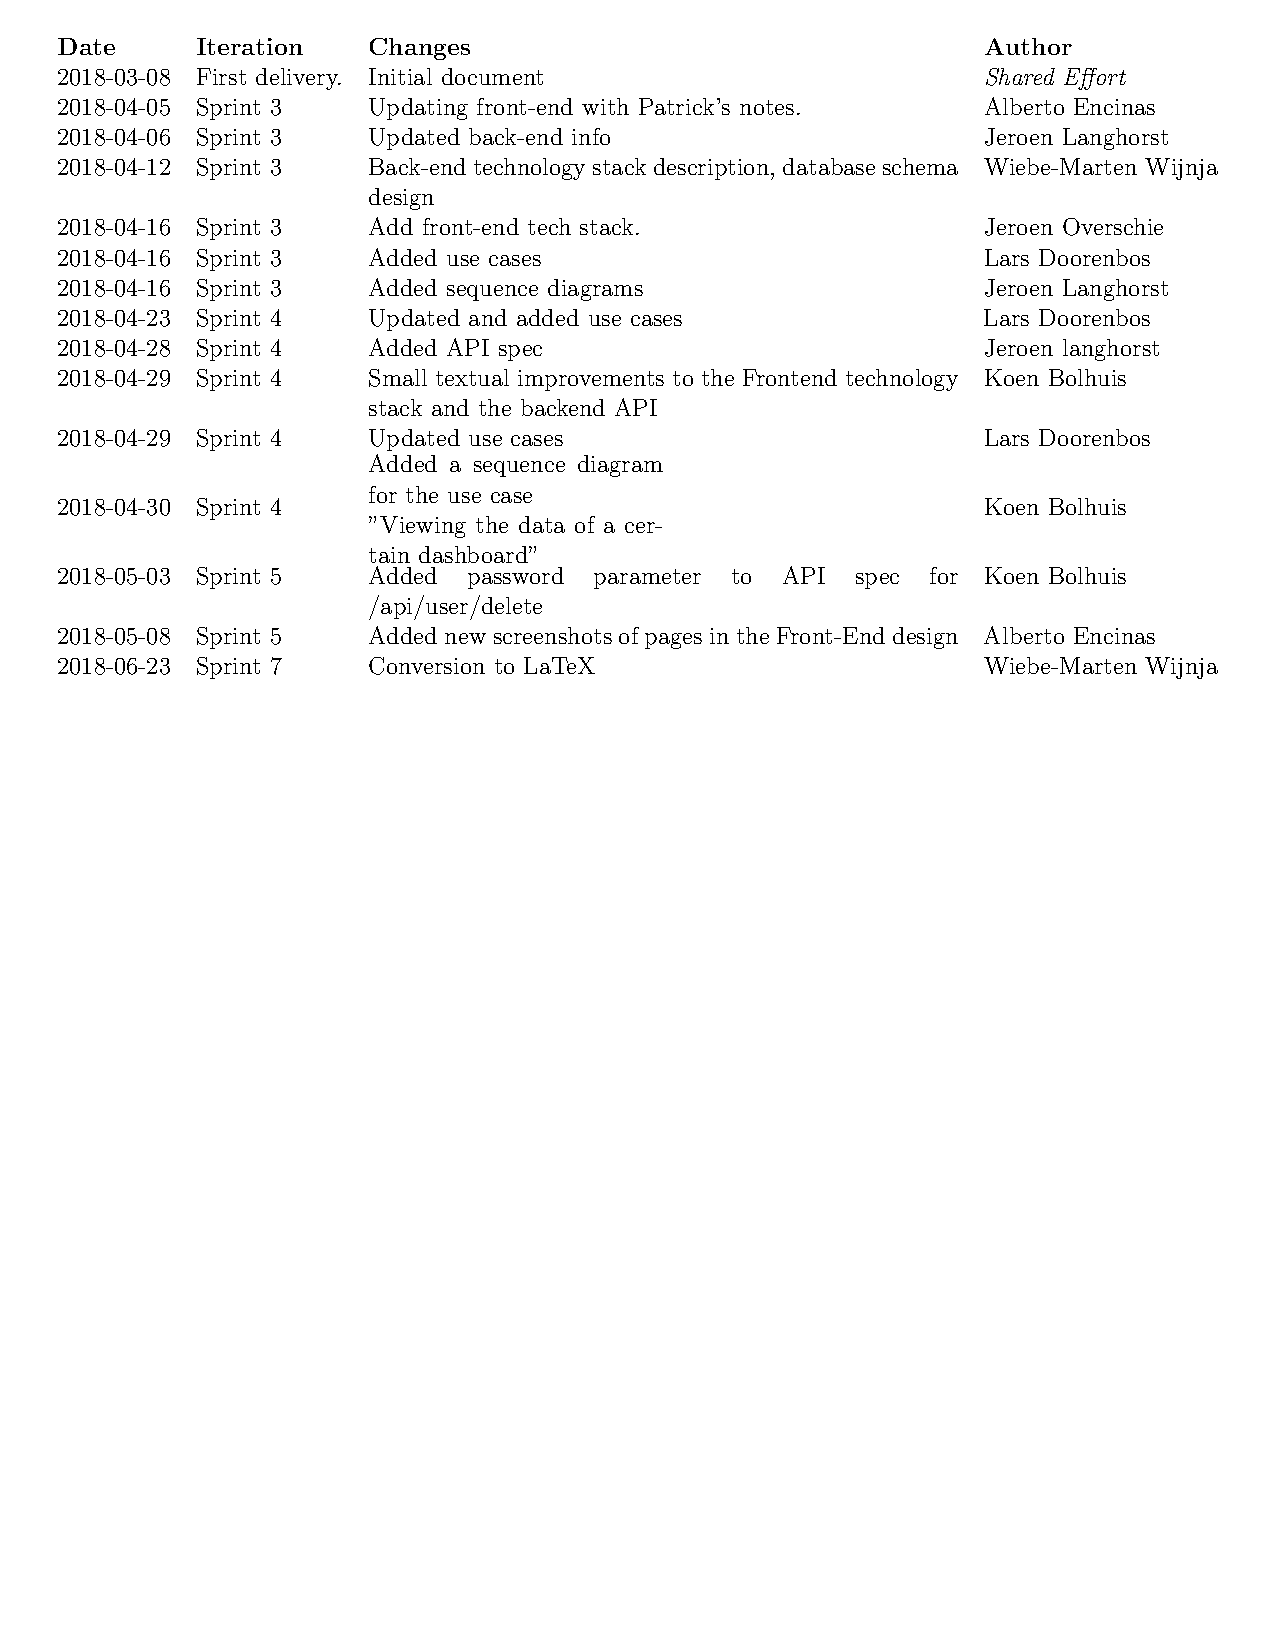
\includegraphics[width=2*\pagewidth]{changelog_architectural.pdf}
